\documentclass[11pt, a4paper]{report}
% ===== ENCODING & LANGUAGE =====
\usepackage[utf8]{inputenc}
\usepackage[T1]{fontenc}
\usepackage[english]{babel}
\usepackage{textcomp}
\usepackage{tikz}
\usetikzlibrary{arrows.meta, positioning, shadows.blur}

% ===== PAGE LAYOUT =====
\usepackage[paperwidth=8.5in,left=1.5in,right=1.0in,top=1.0in,bottom=1.0in,paperheight=11.0in]{geometry}
\usepackage{setspace}
\onehalfspacing
% ===== TEXT ALIGNMENT =====
\usepackage{ragged2e}
\justifying
% ===== GRAPHICS & FIGURES =====
\usepackage{graphicx}
\graphicspath{{./images/}}
\usepackage{float}
\usepackage{caption}
\usepackage{lscape}
\usepackage{pdflscape}
% ===== TABLES =====
\usepackage{longtable}
\usepackage{multirow,bigdelim,dcolumn,booktabs}
% ===== MATH =====
\usepackage{amsmath}
\usepackage{amssymb}
% ===== UNITS =====
\usepackage{siunitx}
% ===== TIKZ & DIAGRAMS =====
\usepackage{tikz}
\usetikzlibrary{shapes.geometric, arrows, decorations.pathreplacing, matrix, positioning, chains}
\usepackage{pgfgantt}
% ===== ALGORITHM =====
\usepackage[ruled,vlined]{algorithm2e}
% ===== CODE LISTINGS =====
\usepackage{listings}
\usepackage{xcolor}
\lstset{
    language=Python,
    basicstyle=\ttfamily\small,
    keywordstyle=\color{blue},
    commentstyle=\color{gray},
    stringstyle=\color{red},
    breaklines=true,
    showstringspaces=false,
    tabsize=4,
    numbers=left,
    numberstyle=\tiny\color{gray},
    frame=single
}
% ===== CITATIONS & REFERENCES =====
\usepackage{cite}
\usepackage{hyperref}
% ===== FORMATTING =====
\usepackage{color}
\usepackage{titlesec}
% ===== CHAPTER FORMATTING =====
\titleformat{\chapter}[display]
  {\normalfont\bfseries\Huge}
  {\chaptertitlename\ \thechapter}{20pt}{\Huge}
\titlespacing*{\chapter}{0pt}{0pt}{40pt}
% ===== NO PARAGRAPH INDENTATION =====
\setlength{\parindent}{0pt}
\setlength{\parskip}{1em}

\begin{document}
\setlength{\parindent}{0pt}
\setlength{\parskip}{2ex plus 0.5ex minus 0.2ex}
\linespread{1.2}
\tolerance2000
\hoffset=-0.5cm
\setlength{\textwidth}{15.5cm}
\setlength{\textheight}{620pt}


\pagestyle{empty}

\begin{center}
\begin{figure}
    \centering
    
\includegraphics[width=0.8\linewidth]{biust.png}
\end{figure}
\vspace*{0.1cm}

{\large \Large \textbf OPTIMIZATION OF TRAFFIC LIGHT CONTROL SYSTEMS FOR
URBAN INTERSECTIONS IN PALAPYE}
\\


\vspace*{1.5cm}

{\large
Full Name: Tsotlhe Nayang Seiphepi\\
Student ID: 21001137\\}
Supervisor : Dr Bokamoso Basutli :  \\
Student Signature:\\
\vspace*{2.0cm}
Supervisor Signature :\\
\vspace*{1.0cm}

EEEN510 - YEAR 5 SEMESTER 1\\
Department of Electrical, Computer and Telecommunications\\
Faculty of Engineering and Technology\\
Botswana International University of Science and Technology\\
Botswana, Palapye

\vspace*{0.2cm}

{\em In partial fulfillment of the requirements for the degree of Bachelor in
Computer and Telecommunications Engineering}

\vspace*{0.2cm}

{\bf 21 November 2025}

\vfill

\end{center}


\newpage
\newpage
\clearpage

% ===== FRONT MATTER =====
\newpage
\pagenumbering{roman}
\onehalfspacing
\tableofcontents
\listoftables
\listoffigures
\newpage

% ===== MAIN CONTENT =====
\pagenumbering{arabic}
\onehalfspacing

\chapter{Introduction}

Palapye is rapidly emerging as both a commercial hub and a strategic transit town, yet its current traffic management system has not kept pace with this growth. The reliance on static, pre-timed traffic signals has become increasingly inadequate in the face of rising vehicular volumes. During peak hours, public holidays, and special events, these systems fail to respond to changing traffic patterns, resulting in chronic congestion, excessive delays, and frustration among commuters.

The consequences go far beyond inconvenience. Prolonged idling leads to higher fuel consumption and air pollution, directly harming the environment and economy. Congestion at busy intersections also increases the likelihood of road accidents, putting public safety at risk. In turn, long and unpredictable waiting times reduce the quality of life for residents and diminish Palapye's attractiveness as a growing urban centre.

These challenges create a strong case for adopting a smarter solution. An intelligent, adaptive traffic control system, capable of adjusting signal timing in real time, offers a path toward safer, cleaner, and more efficient mobility. By reducing delays, improving connectivity, and enhancing overall commuter experience, such a system would not only solve today's pressing traffic issues but also future-proof Palapye's transport network as the town continues to expand.

\section{Background of the study}

Palapye has evolved from a village into a growing town, which is now a very strategically placed settlement. It is situated between Gaborone and Francistown, the two major cities of the country Botswana, connected by the A1 highway. This positioning also makes Palapye a natural gateway for traffic moving between South Africa and Zimbabwe \cite{BIUST_LocateUs}. Major assets such as the Morupule Coal Mine and the Botswana International University of Science and Technology (BIUST) add recurrent, time-peaked demand from shifts, deliveries, and campus activity.

Road capacity and traffic control have not expanded at the same growth rate as the town's activity. Many signalised intersections still run on static, pre-timed cycles that do not respond to fluctuating flows. During peak travel times, public holidays, university openings, and special events, queues build on the A1 road and town access roads, causing longer delays and traffic congestion, higher fuel use, and elevated local gas emissions. Congestion at busy junctions increases crash risk and contributes to commuter frustration, as well as high speeding on the A1 roads as commuters try to reach their delayed destinations earlier. This context motivates a focused study of Palapye's traffic conditions and management options, establishing a baseline against which modern data-driven control strategies can be assessed.

\begin{figure}[H]
  \centering
  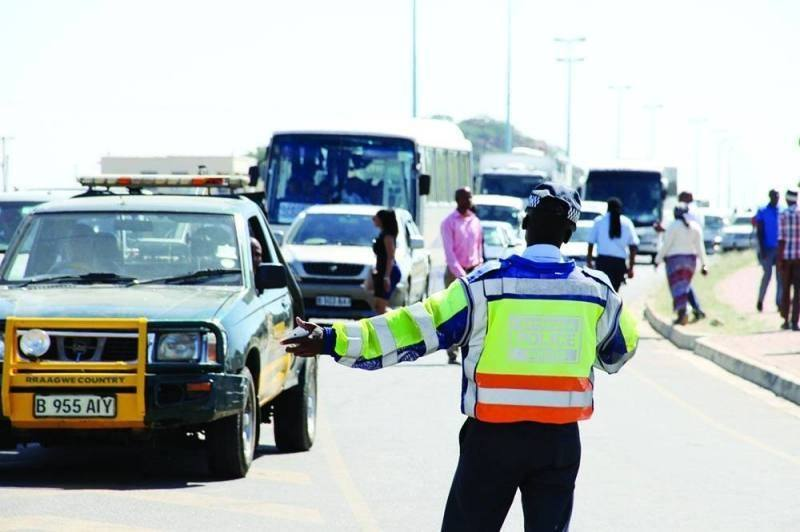
\includegraphics[width=\textwidth]{A1 TRAFFIC.jpg} 
  \caption{Traffic on the A1 road near Palapye (from Mmegi Online) \cite{mmegi_heavy_traffic_a1}}
  \label{fig:traffic_a1}
\end{figure}

\newpage

\section{Problem Statement}

Urban intersections in Palapye experience increased traffic congestion, delays, and inefficient traffic flow due to conventional fixed-time traffic light control systems that do not adapt to real-time traffic conditions.

\newpage

\section{Research Objectives}

\begin{itemize}
    \item Design and implement sensory systems that accurately detect vehicles, pedestrians, and traffic conditions in real time with high reliability and minimal false detection.
    \item Design and implement a networking framework that ensures seamless, low-latency, and secure transmission of traffic data between sensors, local controllers, and the processing unit, supporting both wired and wireless communication protocols.
    \item Design and implement intelligent algorithms that analyse incoming data, optimise signal timing dynamically, and integrate historical traffic patterns to minimise congestion, delay, and emissions while ensuring safety.
    \item Design and implement reliable output control systems that translate optimization decisions into precise operation of traffic signals, pedestrian crossings, and variable message signs in real time.
\end{itemize}

\chapter{Literature Review}

\begin{figure}[H]
    \centering
     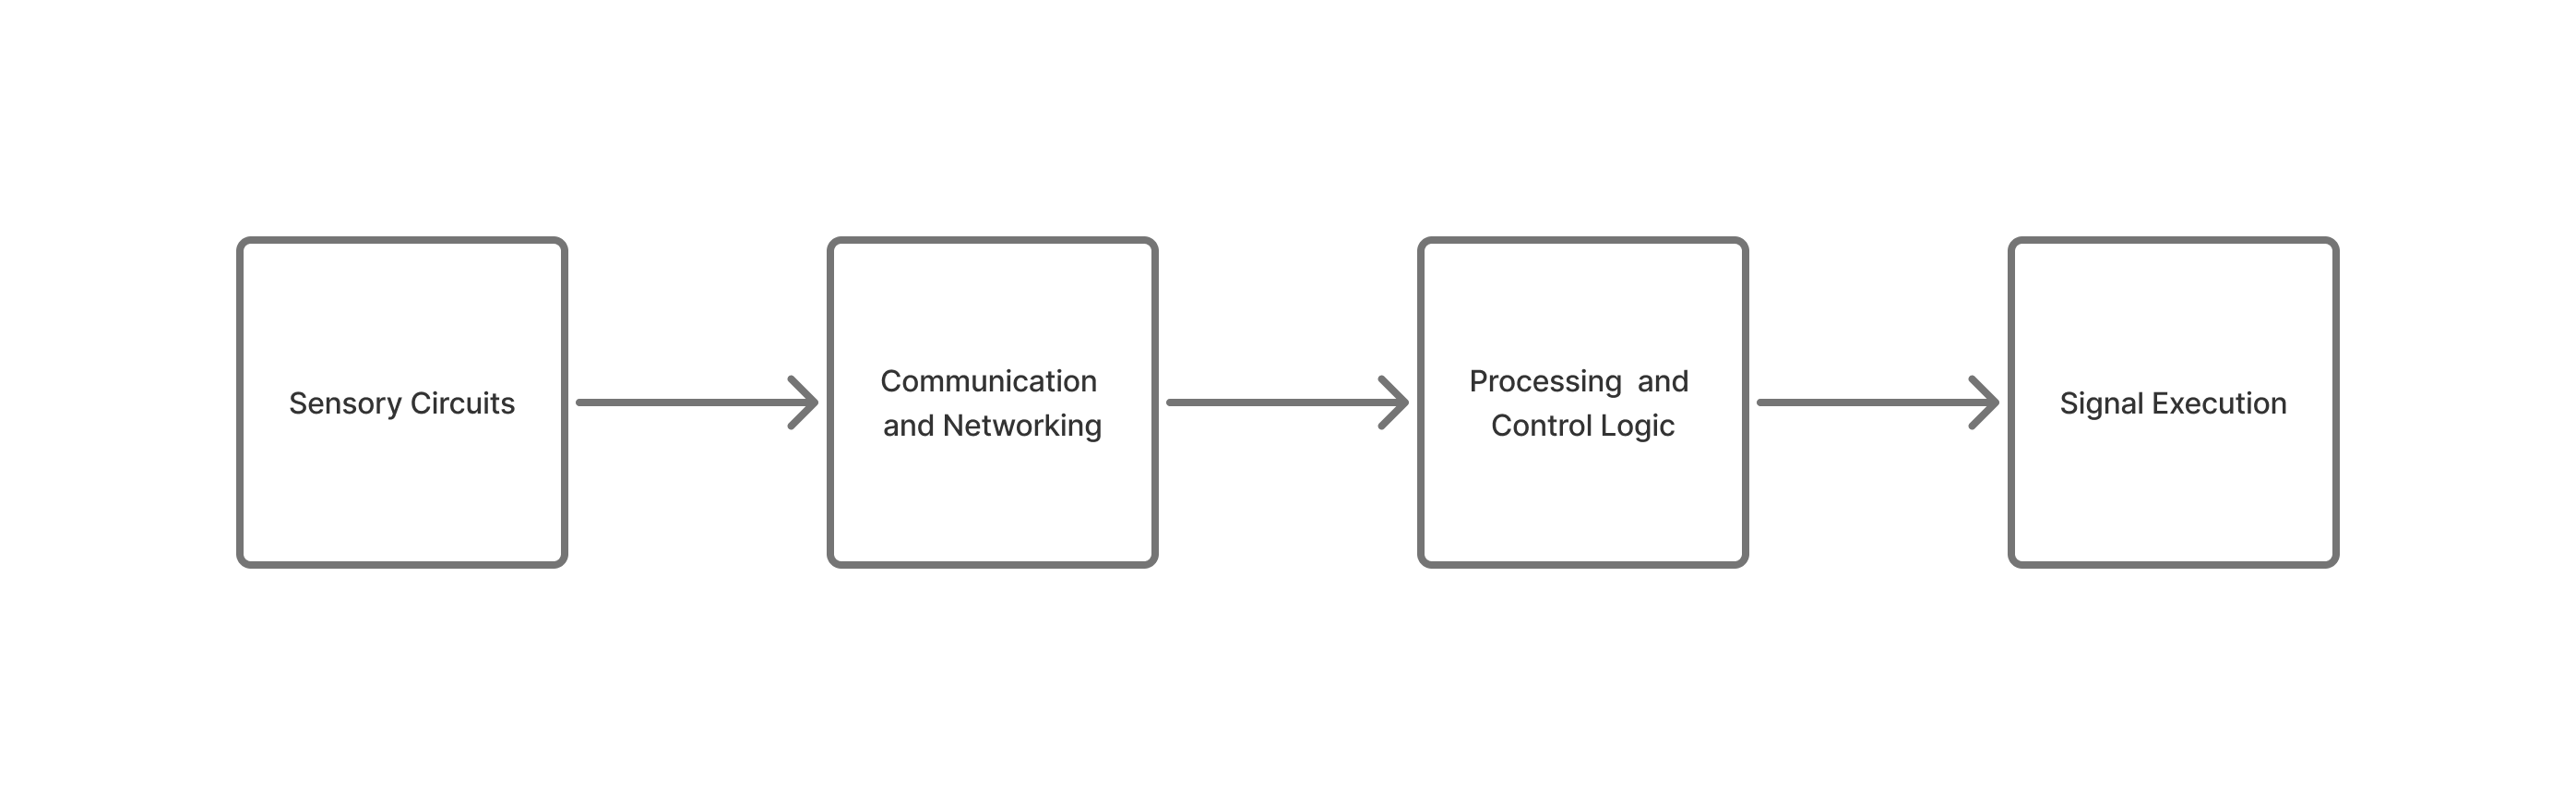
\includegraphics[width=1\linewidth]{Flow chart (Community).png}  
    \caption{Block Diagram of The System}
    \label{fig:block_diagram_system}
\end{figure}

\section{Sensory Circuits}

\textbf{Vehicle Detection using Camera Vision}

The vehicle detection process in the paper by \cite{dos2024vehicular}, is based entirely on classical computer vision techniques implemented using OpenCV. The system begins with video input, where frames are captured from a static camera. Each frame then undergoes background subtraction using the MOG2 algorithm to separate moving objects (vehicles) from the static background. After isolating the moving areas, the image is thresholded and binarized to create a black-and-white mask that clearly distinguishes motion from non-motion regions. Next, the system applies contour detection to identify the outlines of these moving objects. To remove noise and irrelevant small objects, contours below a specific area threshold (e.g., 500--1000 pixels) are discarded, keeping only the larger regions that likely represent vehicles.

For each valid contour, the algorithm computes its centroid (center point) and monitors its position relative to a predefined reference line on the frame. When a centroid crosses this line within a set tolerance range, the system records it as a vehicle count event. This crossing logic ensures each vehicle is counted once as it passes through the scene. The final step updates the vehicle count, allowing the program to estimate traffic flow. According to \cite{dos2024vehicular}, this method achieved high accuracy for smaller vehicles (around 90 percent for cars and 100 percent for motorcycles) but lower accuracy for large vehicles such as buses or trucks due to occlusion and size variability.

\begin{figure}[H]
\begin{center}
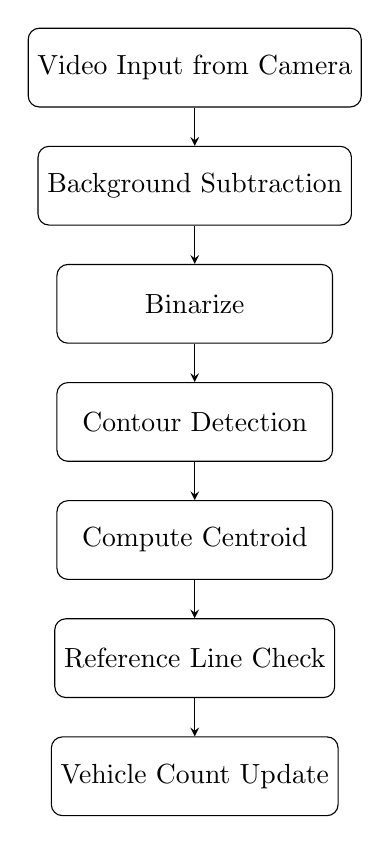
\begin{tikzpicture}[
    node distance=1.5cm,
    every node/.style={rectangle, draw, rounded corners, minimum width=3.5cm, minimum height=1cm, align=center},
    >=stealth
]

% Nodes
\node (input) {Video Input from Camera};
\node (background) [below of=input] {Background Subtraction};
\node (binarize) [below of=background] {Binarize};
\node (contour) [below of=binarize] {Contour Detection};
\node (centroid) [below of=contour] {Compute Centroid};
\node (linecheck) [below of=centroid] {Reference Line Check};
\node (count) [below of=linecheck] {Vehicle Count Update};

% Arrows
\draw [->] (input) -- (background);
\draw [->] (background) -- (binarize);
\draw [->] (binarize) -- (contour);
\draw [->] (contour) -- (centroid);
\draw [->] (centroid) -- (linecheck);
\draw [->] (linecheck) -- (count);

\end{tikzpicture}
\end{center}
\caption{Block diagram of the vehicle detection and counting system.}
\label{fig:vehicle_detection_camera}
\end{figure}

\textbf{Vehicle Detection Using LiDAR}

In the paper ``LiDAR-Enhanced Connected Infrastructures: Sensing and Broadcasting High-Resolution Traffic Information Serving Smart Cities'' \cite{lv2019lidar}, the authors rely entirely on LiDAR sensing to detect, classify, and track vehicles and pedestrians in real time. The LiDAR sensor used---Velodyne VLP-16---emits multiple laser beams that rotate 360 degrees, producing up to 600,000 distance points per second across a range of roughly 100 meters. Each reflected pulse provides a precise 3D coordinate (x, y, z), allowing the system to reconstruct the spatial structure of the road environment. When installed at the roadside about 7--9 feet high, the sensor captures complete 3D profiles of all moving road users within its field of view, independent of light or weather conditions \cite{lv2019lidar}.

The LiDAR system detects vehicles by continuously scanning the surroundings with rotating laser beams that produce a 3D point cloud. Each laser pulse measures the distance to nearby surfaces, so cars appear as dense clusters of reflected points above the ground.

The process starts with background filtering, where stationary objects like roads and buildings are removed using multiple frames to isolate only moving points. Then, DBSCAN clustering groups those remaining points into individual objects based on their spatial density---each cluster likely representing a car, pedestrian, or cyclist. \cite{lv2019lidar}

For every cluster, the system extracts geometric features such as point count, object width, height, and distance from the sensor. These are passed into a Random Forest classifier trained to recognize the difference between vehicles and pedestrians. Vehicles show broader, lower, and denser point distributions than upright, narrow pedestrian clusters.

Once classified, each vehicle's outline is approximated using a minimum-area rectangle, and its motion is tracked frame by frame with Kalman filtering and Global Nearest Neighbor association. This produces a continuous, accurate trajectory for every vehicle within the LiDAR's 100-meter range \cite{lv2019lidar}.

\begin{figure}[H]
\begin{center}
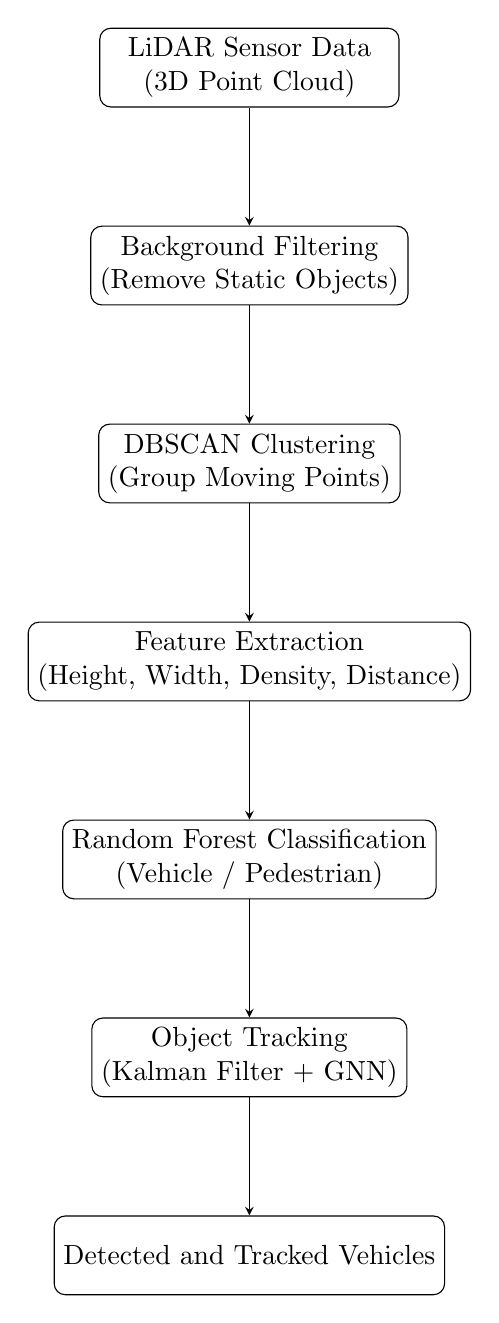
\begin{tikzpicture}[
    node distance=1.5cm,
    every node/.style={rectangle, draw, rounded corners, align=center, minimum width=3.8cm, minimum height=1cm},
    >=stealth
]

% Nodes
\node (input) {LiDAR Sensor Data\\(3D Point Cloud)};
\node (filter) [below=of input] {Background Filtering\\(Remove Static Objects)};
\node (cluster) [below=of filter] {DBSCAN Clustering\\(Group Moving Points)};
\node (features) [below=of cluster] {Feature Extraction\\(Height, Width, Density, Distance)};
\node (classify) [below=of features] {Random Forest Classification\\(Vehicle / Pedestrian)};
\node (track) [below=of classify] {Object Tracking\\(Kalman Filter + GNN)};
\node (output) [below=of track] {Detected and Tracked Vehicles};

% Arrows
\draw[->] (input) -- (filter);
\draw[->] (filter) -- (cluster);
\draw[->] (cluster) -- (features);
\draw[->] (features) -- (classify);
\draw[->] (classify) -- (track);
\draw[->] (track) -- (output);

\end{tikzpicture}
\end{center}
\caption{Block diagram of the LiDAR-based vehicle detection system.}
\label{fig:lidar_detection}
\end{figure}

\textbf{Vehicle Detection Using Radio Waves and Microwaves}

Vehicle detection using radio waves and microwaves represents an emerging technology for traffic monitoring. Radar-based systems operate independently of lighting and weather conditions, providing reliable detection in adverse environments.

\section{Processing and Control Logic}

\subsection{Fixed-Time Control Method}

This technique relies on predetermined schedules for signal phases, where the green, yellow, and red times are fixed in advance. It has been shown to be effective in environments with stable and predictable traffic flows due to its simplicity and ease of implementation. However, the method does not adapt to real-time fluctuations in traffic demand. As a result, its performance deteriorates under conditions of variable density, such as during accidents, special events, or sudden surges in demand \cite{michailidis2025traffic}. There are three common types of fixed-time control methods \cite{tang2019global}:

\begin{enumerate}
    \item \textbf{Isolated Fixed-Time Control}: Each intersection operates on its own predetermined schedule, with no coordination between adjacent intersections.
    \item \textbf{Coordinated Fixed-Time Control}: Intersections are synchronized to create a green wave progression along major corridors, improving traffic flow over longer stretches.
    \item \textbf{Time-of-Day Control}: Signal schedules vary by predefined time periods (e.g., morning peak, off-peak, evening rush), but remain non-responsive to live traffic conditions.
\end{enumerate}

\subsection{Actuated Control Method}

The actuated control method adjusts signal timings dynamically based on real-time inputs from sensors such as loop detectors, cameras, and infrared devices \cite{kalavsova2022impact}. Unlike fixed-time systems, which rely on predetermined schedules, actuated control responds directly to actual vehicle arrivals by extending green phases when vehicles are detected within the extension window. This responsiveness improves intersection efficiency by reducing unnecessary idling and abrupt stops.

Kalašová \cite{kalavsova2022impact} investigated the impact of actuated signal control on both traffic flow and environmental outcomes. Their evaluation focused on key performance indicators, including average delay, queue length, fuel consumption, and emissions. The average delay per vehicle was defined as:

\begin{equation}
d = \frac{\sum (t_{\text{actual}} - t_{\text{free}})}{N}
\label{eq:average-delay}
\end{equation}

where $t_{\text{actual}}$ is the actual travel time, $t_{\text{free}}$ is the free-flow travel time, and $N$ is the number of vehicles observed.

Queue length was measured as the accumulation of vehicles at red signals, while environmental indicators such as fuel consumption and emissions were modeled as functions of idling time and acceleration cycles.

The study showed that actuated control, which adjusts traffic signals based on real-time traffic, significantly cuts down on delays and queue lengths compared to fixed-time signals, especially in variable or moderate traffic conditions. It also reduces idling and stop-and-go driving, leading to lower CO$_2$ emissions and fuel use. However, in heavily congested, over saturated conditions, actuated control alone is not enough to fully resolve congestion or delays.

Overall, research highlights actuated signal control as a substantial improvement over fixed-time methods, especially in urban environments where traffic demand fluctuates throughout the day \cite{kalavsova2022impact}.

\subsection{Adaptive Control Method}

The adaptive control method represents the latest and most advanced form of traffic signal management. They continuously monitor traffic density in real time and apply algorithmic models to optimize signals across networks \cite{mannion2016experimental}. The adaptive models reduce traffic delays and adapt to real time traffic densities. The adaptive models are divided into two types \cite{ye2019survey}.

\section{Model-Based Optimization Systems}

These systems use mathematical models to represent how traffic behaves. Instead of trial and error, they predict what traffic will look like and then decide the best traffic signal timings. Common approaches include:

\subsection{Model Predictive Control}

This technique predicts future traffic states like queue lengths and delays over a finite prediction horizon and computes the best signal timings in advance. A mathematical model predicts how traffic will evolve if certain green/red timings are applied. An optimization problem is solved to minimize a cost function subject to constraints like minimum green time or safety rules. The first part of the optimized signal plan is implemented. The process repeats at the next step with updated traffic data \cite{8707103}. Mathematically, the MPC problem is expressed as:

\begin{equation}
\min_{u(0), \dots, u(N-1)} \sum_{k=0}^{N-1} J(x(k), u(k)) + J_f(x(N))
\label{eq:mpc-objective}
\end{equation}

subject to:

\begin{equation}
x(k+1) = f(x(k), u(k)) + d(k), \quad x(k) \in X, \; u(k) \in U
\label{eq:mpc-constraint}
\end{equation}

where:

\begin{itemize}
    \item $x(k)$ represents the traffic state (e.g., queue lengths or densities)
    \item $u(k)$ is the control action (signal timings)
    \item $d(k)$ is the demand disturbance
\end{itemize}

The stage cost $J(x,u)$ typically combines queue lengths, waiting times, or number of stops, while $J_f(x(N))$ serves as a terminal cost penalizing undesirable end states.

\cite{8707103} found out that MPC can anticipate future conditions, explicitly handle multi-variable intersections and constraints, and achieves better performance compared to fixed and actuated control strategies. Distributed and hierarchical MPC variants also offer improved coordination among multiple intersections.

However \cite{8707103} highlighted critical limitations of the MPC. Centralized MPC is poor at computational complexity that restricts real time feasibility in large urban networks, performance is highly dependent on the accuracy of traffic models, and most applications remain at the simulation stage, with few large-scale real-world deployments. Scalability and robustness to uncertainty remain open challenges \cite{8707103}.

\subsection{Dynamic Traffic Assignment (DTA)}

Dynamic Traffic Assignment (DTA) extends static traffic assignment by considering the time-varying nature of traffic demand and network conditions. The goal is to allocate vehicles dynamically across available routes to minimize congestion and balance traffic loads. Unlike static methods, which assume fixed flows, DTA accounts for fluctuations in demand, travel times, and congestion propagation throughout the network. This makes it suitable for analyzing real-world urban environments where traffic conditions evolve continuously \cite{elimadi2024review}.

Dynamic Traffic Assignment (DTA) is often formulated as a Dynamic User Equilibrium (DUE), where no driver can improve their travel time by unilaterally changing routes. The optimization problem can be expressed as \cite{elimadi2024review}:

\begin{equation}
\min_{x} \sum_{a \in A} \int_{0}^{x_a(t)} c_a(s)\,ds
\label{eq:dta-objective}
\end{equation}

subject to:

\begin{equation}
\sum_{p \in P_{od}} h_p(t) = d_{od}(t), \quad \forall (o,d) \in OD
\label{eq:dta-constraint}
\end{equation}

where:

\begin{itemize}
    \item $x_a(t)$ is the flow on link $a$ at time $t$
    \item $c_a(s)$ is the travel cost (delay) on link $a$ as a function of flow
    \item $h_p(t)$ is the departure rate on path $p$
    \item $d_{od}(t)$ is the time-dependent travel demand between origin $o$ and destination $d$
\end{itemize}

At user equilibrium, all routes used between an origin--destination pair have equal and minimal travel times, meaning no individual driver can reduce their travel time by switching routes.

The findings of the paper \cite{elimadi2024review} indicated that the DTA can model how drivers change routes over time and how congestion builds across a city. It shows where traffic will flow, where bottlenecks form and how control strategies affect the whole system. Best use case for planning, tolling, ramp metering and signal coordination. However limitations of the model indicate that it needs detailed forecasts and accurate models of driver behavior which are very hard to obtain. It becomes computationally heavy in larger cities, making real time use difficult. The model does not handle unexpected results such as accidents and sudden traffic.

\subsection{Mixed-Integer Linear Programming (MILP)}

This approach formulates the problem of scheduling green, yellow, and red phases as a set of linear equations and inequalities, with decision variables representing signal timings. Some variables are continuous (e.g., cycle lengths, green time durations), while others are integer or binary (e.g., whether a phase is active at a given time) \cite{guilliard2016nonhomogeneous}.

The general form of a Mixed-Integer Linear Program (MILP) can be expressed as \cite{ye2019survey}:

\begin{equation}
\min_{x} \; c^T x
\label{eq:milp-objective}
\end{equation}

subject to:

\begin{equation}
Ax \leq b
\label{eq:milp-constraint1}
\end{equation}

\begin{equation}
x_i \in \mathbb{Z}, \quad x_j \in \mathbb{R}
\label{eq:milp-constraint2}
\end{equation}

where:

\begin{itemize}
    \item $x$ is the decision vector (e.g., vehicle scheduling times, phase activations)
    \item $c$ is the cost vector (e.g., delays or travel times)
    \item $A$ is the constraint matrix and $b$ is the constraint bound
    \item $x_i \in \mathbb{Z}$ represent integer/binary decision variables (e.g., sequencing orders)
    \item $x_j \in \mathbb{R}$ represent continuous decision variables (e.g., timing values)
\end{itemize}

In the context of traffic control, \cite{ye2019survey} formulated the MILP objective to minimize total delay of vehicles crossing an intersection, subject to linear constraints ensuring safety gaps, collision avoidance, and signal timing requirements.

Their findings from their research indicated that there was significant delay and stop reduction. In one simulation scenario, only 11 cars were forced to stop under the MILP scheme versus 1162 under a baseline fixed-time signal \cite{ye2019survey}. The other findings were that it is feasible in real-time computation.

However the limitations include scalability in large networks making computational very difficult. It is run under assumptions that are not applicable in the real world for example, they ignored left and right turns in their formulation to simplify the model \cite{ye2019survey}.

\section{Model-free Optimization Systems}

These systems, instead of predicting traffic through mathematical models, learn directly from real traffic data. This data is gathered from datasets and live sensors. They adapt based on experience. Common approaches include:

\begin{itemize}
    \item Reinforcement Learning
    \item Fuzzy Logic
    \item Evolutionary Algorithms
    \item Swarm Intelligence
\end{itemize}

\subsection{Reinforcement Learning}

It is a model free optimization technique that enables an artificial agent to learn optimal traffic signal control strategies through trial and error interaction with the environment. Unlike model-based methods such as MPC or DTA, it does not require explicit traffic flow equations. Instead it uses real time feedback such as queue lengths, waiting times and vehicle delayed which uses them to determine feedback actions which are signal phase changes that maximize long term performance \cite{futuretransp5040137}.

RL systems consist of 4 key elements: state, action, reward and policy. The state represents the current traffic condition, the action represents the selected control decision and the reward quantifies the benefit of the chosen action. The policy maps states to action and is improved iteratively through learning \cite{futuretransp5040137}.

\begin{figure}[H]
    \centering
     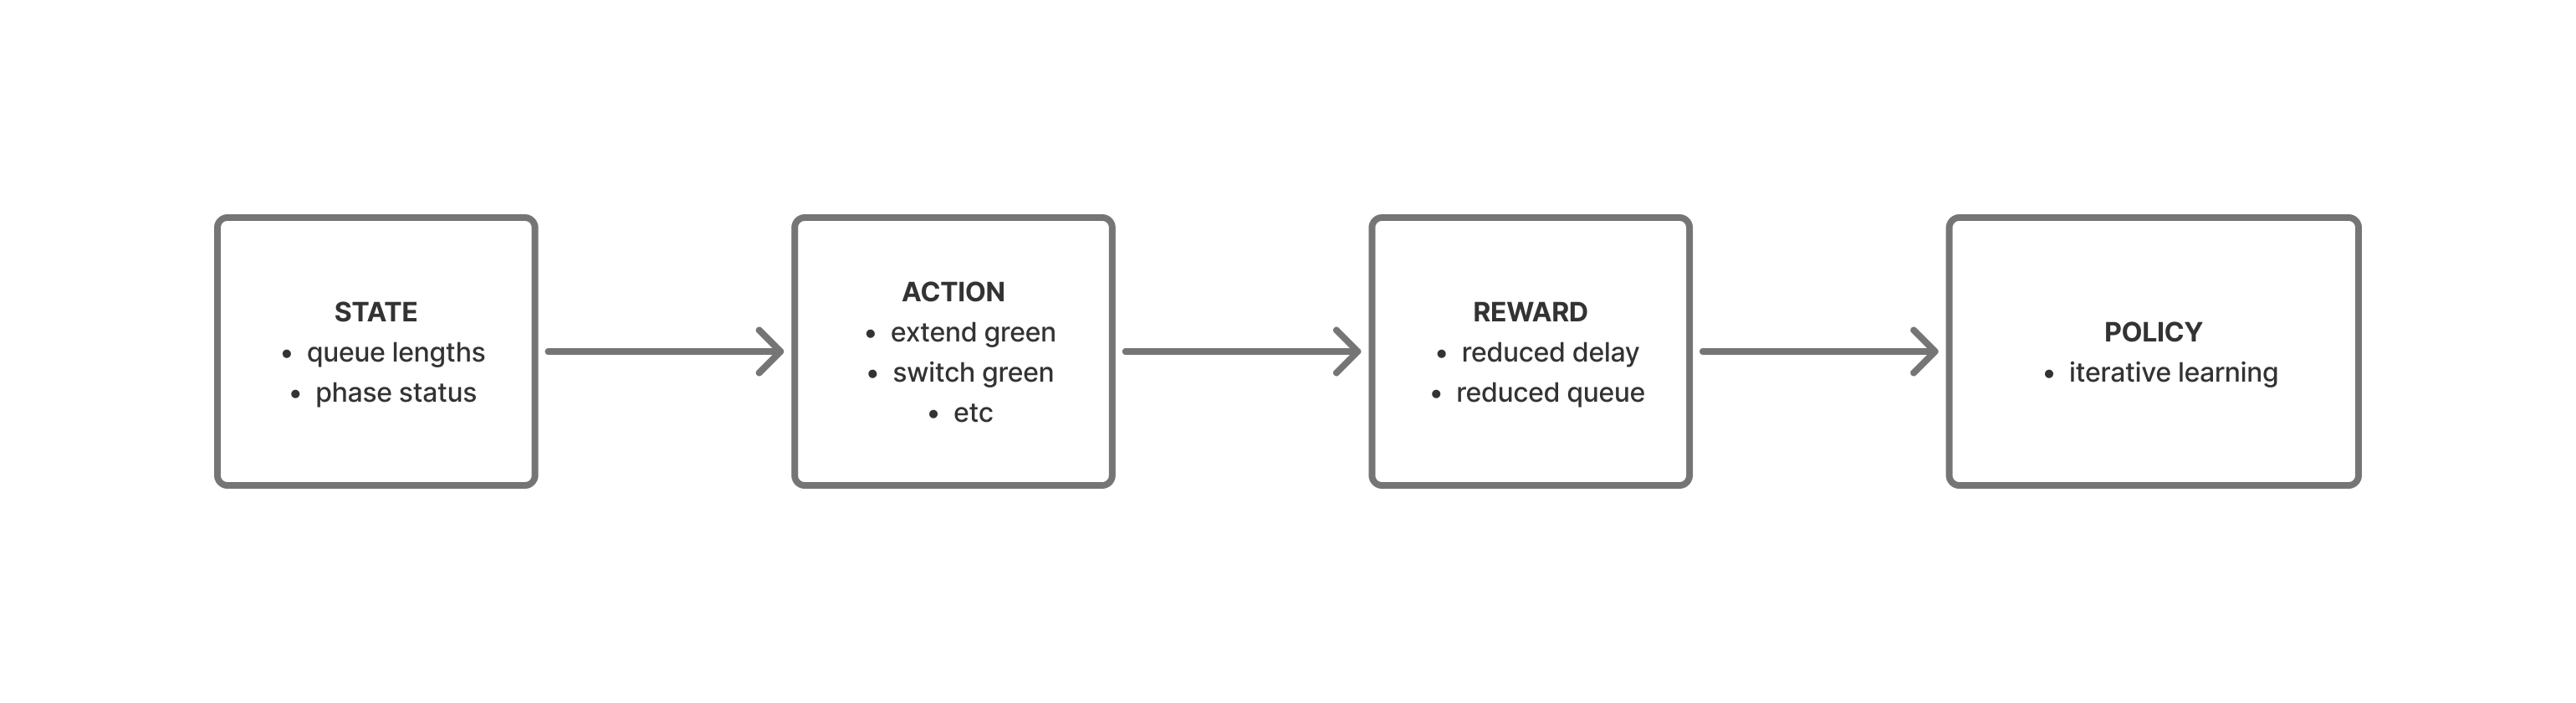
\includegraphics[width=1\linewidth]{Flow chart (Community) (3).png}  
    \caption{Block Diagram of Reinforcement Learning System}
    \label{fig:reinforcement_learning_block}
\end{figure}

\subsection{Reinforcement Learning (RL) Update Rule}

The Q-learning algorithm updates its knowledge of the optimal policy through the following recursive relation:

\begin{equation}
Q(s,a) \leftarrow Q(s,a) + \alpha \big[ r + \gamma \max_{a'} Q(s',a') - Q(s,a) \big]
\end{equation}

where:

\begin{itemize}
    \item $Q(s,a)$ represents the value of taking action $a$ in state $s$
    \item $\alpha$ is the learning rate that controls how much new information overrides old estimates
    \item $\gamma$ is the discount factor determining the importance of future rewards
    \item $r$ is the immediate reward received after taking action $a$
    \item $s'$, $a'$ denote the next state and action
\end{itemize}

This equation enables the learning agent to iteratively improve its policy by updating the estimated value of each state--action pair based on observed rewards. The algorithm updates its knowledge until convergence toward an optimal policy that minimizes total traffic delay or maximizes throughput.

Variants such as Deep Q-Networks (DQN), Actor--Critic (A2C, A3C), Proximal Policy Optimization (PPO), and Multi-Agent RL extend this framework to complex, multi-intersection environments.

\subsubsection{Reinforcement Learning Models}

Reinforcement Learning (RL) has emerged as one of the most effective model-free optimization approaches in traffic signal control. Unlike model-based controllers, which rely on fixed mathematical descriptions of traffic flow, RL agents learn control strategies directly through repeated interaction with the environment. This allows an RL controller to adapt to irregular traffic patterns, unforeseen disturbances, and non-linear flow characteristics that conventional models cannot explicitly describe \cite{futuretransp5040137}.

In the RL framework, traffic control is represented as a Markov Decision Process (MDP). At each decision step, the controller observes the current traffic state $s_t$, selects a signal action $a_t$, receives a reward $r_t$ based on system performance, and transitions to a new state $s_{t+1}$. Over time, the agent learns a policy $\pi(a|s)$ that maximizes expected cumulative reward. Figure \ref{fig:rl_overall_block} illustrates the high-level RL control loop.

\begin{figure}[H]
\centering
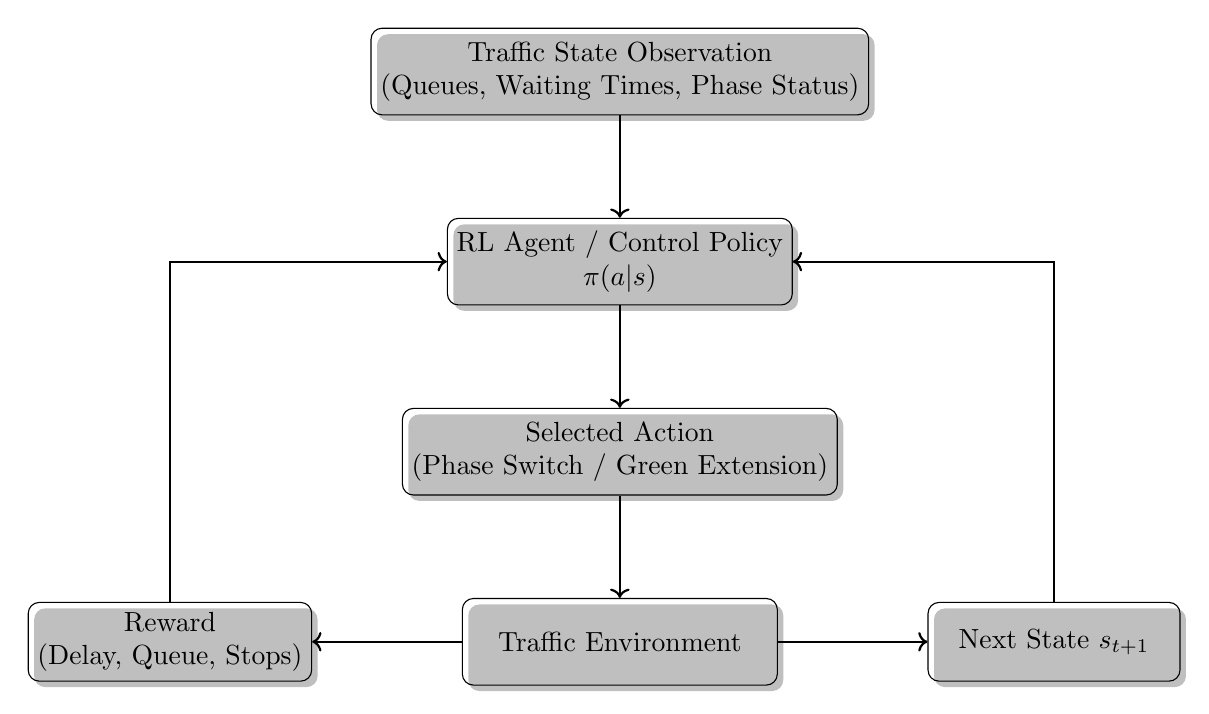
\begin{tikzpicture}[
    node distance=1.3cm,
    block/.style={rectangle, draw, rounded corners, minimum width=4.0cm, minimum height=1.1cm, align=center, drop shadow},
    smallblock/.style={rectangle, draw, rounded corners, minimum width=3.2cm, minimum height=1cm, align=center, drop shadow},
    arrow/.style={->, thick},
]

% Main vertical flow
\node[block] (state) {Traffic State Observation\\(Queues, Waiting Times, Phase Status)};
\node[block, below=of state] (policy) {RL Agent / Control Policy\\$\pi(a|s)$};
\node[block, below=of policy] (action) {Selected Action\\(Phase Switch / Green Extension)};
\node[block, below=of action] (environment) {Traffic Environment};

% Side nodes
\node[smallblock, left=1.9cm of environment] (reward) {Reward\\(Delay, Queue, Stops)};
\node[smallblock, right=1.9cm of environment] (nextstate) {Next State $s_{t+1}$};

% Arrows
\draw[arrow] (state) -- (policy);
\draw[arrow] (policy) -- (action);
\draw[arrow] (action) -- (environment);

\draw[arrow] (environment) -- (reward);
\draw[arrow] (environment) -- (nextstate);

\draw[arrow] (reward) |- (policy);
\draw[arrow] (nextstate) |- (policy);

\end{tikzpicture}
\caption{High-level RL control loop for adaptive traffic signal control.}
\label{fig:rl_overall_block}
\end{figure}

\paragraph{Deep Q-Learning (DQN)}

Deep Q-Learning is a value-based RL algorithm that approximates the action-value function $Q(s,a)$ using a deep neural network. It is effective for traffic signal control where actions (e.g., selecting the next phase) are discrete. The Q-function is updated using the Bellman equation:

\begin{equation}
Q(s,a) \leftarrow Q(s,a) + \alpha \left[r + \gamma \max_{a'}Q(s',a') - Q(s,a)\right]
\label{eq:dqn}
\end{equation}

To enhance stability, DQN employs experience replay and a target network that updates slowly. Figure \ref{fig:dqn_block} shows the improved systems-engineering diagram for the DQN workflow.

\begin{figure}[H]
\centering
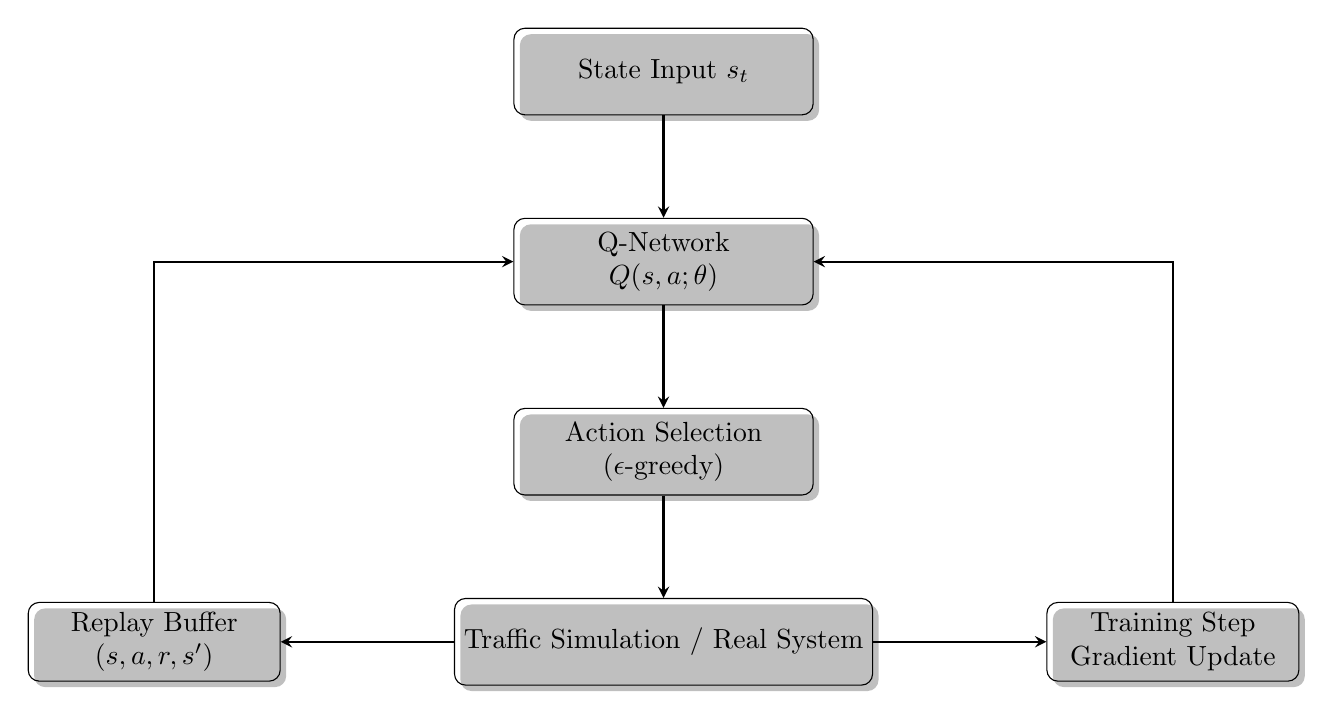
\begin{tikzpicture}[
    node distance=1.3cm,
    block/.style={
        rectangle, draw, rounded corners,
        minimum width=3.8cm, minimum height=1.1cm,
        align=center, drop shadow
    },
    sideblock/.style={
        rectangle, draw, rounded corners,
        minimum width=3.2cm, minimum height=1.0cm,
        align=center, drop shadow
    },
    arrow/.style={-stealth, thick}
]

% Main vertical blocks
\node[block] (state) {State Input $s_t$};
\node[block, below=of state] (qnet) {Q-Network\\$Q(s,a;\theta)$};
\node[block, below=of qnet] (act) {Action Selection\\($\epsilon$-greedy)};
\node[block, below=of act] (env) {Traffic Simulation / Real System};

% Side blocks
\node[sideblock, left=2.2cm of env] (buffer) {Replay Buffer\\$(s,a,r,s')$};
\node[sideblock, right=2.2cm of env] (train) {Training Step\\Gradient Update};

% Main arrows
\draw[arrow] (state) -- (qnet);
\draw[arrow] (qnet) -- (act);
\draw[arrow] (act) -- (env);

% Side arrows
\draw[arrow] (env.west) -- (buffer.east);
\draw[arrow] (buffer.north) |- (qnet.west);

\draw[arrow] (env.east) -- (train.west);
\draw[arrow] (train.north) |- (qnet.east);

\end{tikzpicture}
\caption{DQN architecture for traffic signal decision-making.}
\label{fig:dqn_block}
\end{figure}

\paragraph{Proximal Policy Optimization (PPO)}

PPO is an actor--critic method known for its stability and strong performance in continuous and discrete action environments. It updates the policy using a clipped surrogate objective to prevent destructive updates:

\begin{equation}
\mathcal{L}^{\text{CLIP}} = 
\mathbb{E}\left[\min\left(
r_t(\theta)\hat{A}_t,\;\;
\text{clip}(r_t(\theta),1-\epsilon,1+\epsilon)\hat{A}_t
\right)\right]
\label{eq:ppo}
\end{equation}

where $r_t(\theta)=\frac{\pi_{\theta}(a_t|s_t)}{\pi_{\theta_{\text{old}}}(a_t|s_t)}$ is the probability ratio. Figure \ref{fig:ppo_block} shows the PPO system architecture.

\begin{figure}[H]
\centering
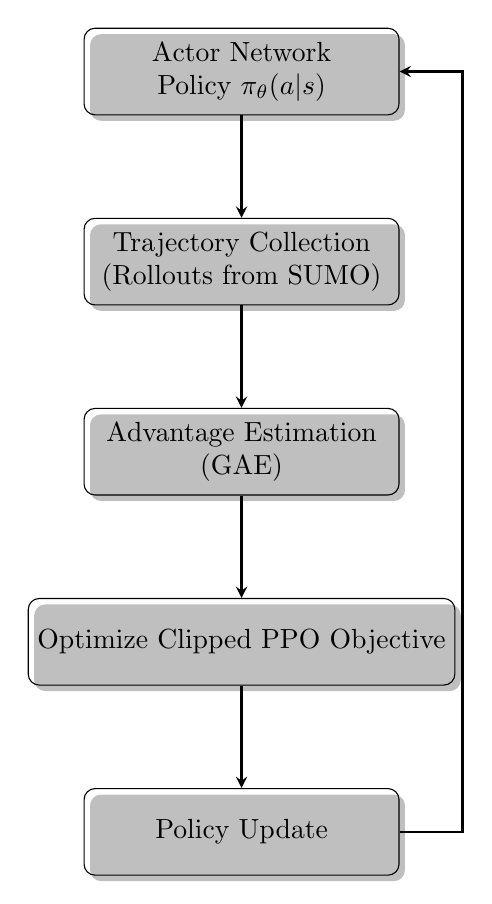
\begin{tikzpicture}[
    node distance=1.3cm,
    block/.style={
        rectangle, draw, rounded corners,
        minimum width=4.0cm, minimum height=1.1cm,
        align=center, drop shadow
    },
    arrow/.style={-stealth, thick},
]

% Main vertical flow
\node[block] (actor) {Actor Network\\Policy $\pi_\theta(a|s)$};
\node[block, below=of actor] (roll) {Trajectory Collection\\(Rollouts from SUMO)};
\node[block, below=of roll] (adv) {Advantage Estimation\\(GAE)};
\node[block, below=of adv] (opt) {Optimize Clipped PPO Objective};
\node[block, below=of opt] (update) {Policy Update};

% Vertical arrows
\draw[arrow] (actor) -- (roll);
\draw[arrow] (roll) -- (adv);
\draw[arrow] (adv) -- (opt);
\draw[arrow] (opt) -- (update);

% Clean loopback arrow
\draw[arrow] (update.east) -| ([xshift=0.8cm]actor.east) -- (actor.east);

\end{tikzpicture}
\caption{Proximal Policy Optimization (PPO) workflow.}
\label{fig:ppo_block}
\end{figure}

\paragraph{Continuous Control Models (DDPG, TD3, SAC)}

For green-time allocation where actions are continuous, deterministic or stochastic actor--critic algorithms are used:

\begin{itemize}
    \item \textbf{DDPG} --- deterministic signal policy; useful but unstable.
    \item \textbf{TD3} --- improves DDPG via clipped double Q-learning.
    \item \textbf{SAC} --- adds entropy regularization for robust exploration.
\end{itemize}

These methods allow the agent to choose precise green durations instead of discrete phase selections.

\subsection{Multi-agent reinforcement learning for traffic signal control}

When a road network has multiple signalised intersections close together, what one junction does immediately affects the next. Add more green time at intersection A and you push a wave of vehicles toward B, which may not be ready for them. Managing all signals through one joint action space quickly becomes impractical — the action space grows exponentially with each intersection added \cite{busoniu2008comprehensive}. Multi-Agent Reinforcement Learning (MARL) assigns a separate agent to each intersection, keeping the problem tractable while still allowing coordination across the network.

\subsubsection{The centralised-decentralised spectrum}

MARL approaches differ mainly in how much information agents share during training and at runtime. At one end, a single controller sees the entire network. At the other, each agent is on its own. Both cause problems.

\paragraph{Fully centralised control}

A centralised controller observes the full network state and outputs a joint action for all intersections. In theory this finds the globally optimal policy, but the joint state and action spaces grow combinatorially with every junction added, so training becomes computationally infeasible beyond a small network \cite{mannion2016experimental}. There is also a deployment problem: all sensor data has to reach one processing unit in real time, which introduces latency and creates a single point of failure.

\paragraph{Fully decentralised control -- independent learning}

At the other extreme, each agent treats the others as part of the environment and learns entirely on its own local observations. Independent Q-Learning (IQL), where each intersection runs a standard DQN, is the simplest version. The difficulty is that all agents' policies are changing simultaneously during training, so the environment looks non-stationary from any one agent's perspective. This breaks the Markov assumption that Q-learning depends on, causing training to oscillate or fail to converge \cite{tan1993multi}. In traffic networks, independent agents reliably find locally rational but globally harmful strategies. One intersection holds green longer to clear its own queue while pushing vehicles into the next junction, making delay worse across the network.

\subsubsection{Centralised training with decentralised execution (CTDE)}

CTDE, formalised by \cite{oliehoek2008optimal} and made widely known through MADDPG \cite{lowe2017multi}, separates what is needed at training time from what is needed at deployment. The restriction on information sharing only applies when the system is running in the real world. During training, which happens entirely in simulation, agents can share whatever is useful.

Each agent keeps a local policy — the Actor — that takes only its own observations as input. This is what runs on the deployed system. A centralised value function — the Critic — is trained on the full joint state of all agents and is only used during training. Once training ends, the Critic is discarded. Every intersection then runs its Actor on local sensor data alone.

\begin{figure}[H]
\centering
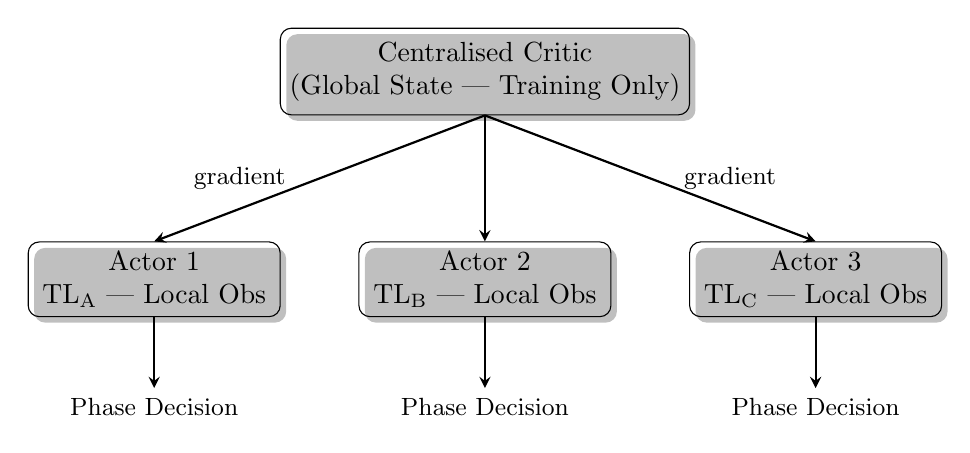
\begin{tikzpicture}[
    node distance=1.1cm,
    block/.style={
        rectangle, draw, rounded corners,
        minimum width=4.5cm, minimum height=1.1cm,
        align=center, drop shadow
    },
    agent/.style={
        rectangle, draw, rounded corners,
        minimum width=3.2cm, minimum height=0.9cm,
        align=center, drop shadow
    },
    arrow/.style={-stealth, thick},
]

\node[block] (critic) {Centralised Critic\\(Global State --- Training Only)};

\node[agent, below=1.6cm of critic, xshift=-4.2cm] (a1) {Actor 1\\TL\textsubscript{A} --- Local Obs};
\node[agent, below=1.6cm of critic]                (a2) {Actor 2\\TL\textsubscript{B} --- Local Obs};
\node[agent, below=1.6cm of critic, xshift= 4.2cm] (a3) {Actor 3\\TL\textsubscript{C} --- Local Obs};

\draw[arrow] (critic.south) -- (a1.north) node[midway, left=0.3cm]{\small gradient};
\draw[arrow] (critic.south) -- (a2.north);
\draw[arrow] (critic.south) -- (a3.north) node[midway, right=0.3cm]{\small gradient};

\draw[arrow] (a1.south) -- ++(0,-0.9) node[below]{\small Phase Decision};
\draw[arrow] (a2.south) -- ++(0,-0.9) node[below]{\small Phase Decision};
\draw[arrow] (a3.south) -- ++(0,-0.9) node[below]{\small Phase Decision};

\end{tikzpicture}
\caption{Centralised training with decentralised execution. The Critic uses global state during training to guide all Actors; only the local Actors run at deployment.}
\label{fig:ctde_diagram}
\end{figure}

Because the Critic observes all agents at once, it operates in a stationary joint environment, which is what the independent learning approach breaks. Each Actor receives stable gradient signals during training even though it only ever sees its own local data \cite{lowe2017multi}.

\subsubsection{Key CTDE algorithms}

\paragraph{MADDPG}

Lowe et al.\ \cite{lowe2017multi} extended DDPG to the multi-agent setting by giving each agent its own centralised critic conditioned on all agents' observations and actions. It was among the first algorithms to show that CTDE could handle cooperative and competitive tasks in continuous action spaces. It does inherit DDPG's training instability, and maintaining a separate critic per agent becomes expensive as the network grows.

\paragraph{QMIX}

QMIX \cite{rashid2018qmix} decomposes the joint action-value function $Q_{tot}$ into per-agent values $Q_i$ through a mixing network, under a monotonicity constraint:
\begin{equation}
\frac{\partial Q_{tot}}{\partial Q_i} \geq 0 \quad \forall i
\label{eq:qmix_monotone}
\end{equation}
This guarantees that the action each agent picks independently is also the globally optimal joint action, so decentralised execution is safe. QMIX showed strong results on the StarCraft Multi-Agent Challenge \cite{samvelyan2019starcraft} and has been applied to traffic signal control with discrete action spaces.

\paragraph{MAPPO}

Yu et al.\ \cite{yu2022surprising} showed that extending PPO directly to cooperative multi-agent settings --- MAPPO --- matches or beats more specialised algorithms including QMIX across a range of benchmarks. Each agent has its own Actor on local observations; a single shared Critic takes the concatenated global state of all agents. The PPO clipped objective applies to each agent with a shared advantage estimate:
\begin{equation}
\mathcal{L}^{\text{CLIP}}_i = \mathbb{E}\left[\min\left(r_i(\theta)\hat{A}, \;\text{clip}(r_i(\theta), 1-\epsilon, 1+\epsilon)\hat{A}\right)\right]
\label{eq:mappo_clip}
\end{equation}

where $r_i(\theta) = \frac{\pi_\theta(a_i | o_i)}{\pi_{\theta_\text{old}}(a_i | o_i)}$ is the probability ratio for agent $i$, and $\hat{A}$ is the advantage estimated from the centralised critic via GAE \cite{schulman2015high}. The result from \cite{yu2022surprising} is that PPO's simplicity is not a weakness --- a well-tuned shared critic with normalised advantages is enough to get strong cooperative performance without the added complexity of value decomposition.

\subsubsection{Parameter sharing}

When all agents observe the same feature types and choose from the same action space --- as is the case for a network of similar intersections --- they can share Actor network weights. Training uses experience from all agents simultaneously, which multiplies the effective batch size and tends to produce more stable gradients than training separate networks per agent \cite{gupta2017cooperative}. It also reduces the total number of parameters, making training faster.

\subsubsection{Cooperative reward design}

How the reward is defined has a large effect on whether agents learn to cooperate or compete \cite{chu2019multi}. Three approaches appear in the literature:

\begin{enumerate}
    \item Local reward: each agent gets a reward based on its own intersection only. Simple to compute, but leads to selfish behaviour --- one agent may extend green to clear its own queue while pushing vehicles into the next junction.
    \item Global reward: all agents share one reward computed across the whole network, such as total waiting time. This targets network-level cooperation directly, but makes it harder for any single agent to trace which of its actions contributed to the outcome.
    \item Mixed reward: a weighted combination of the two.
\end{enumerate}

Traffic signal control studies find that a global reward, paired with a centralised critic to handle credit assignment, consistently produces better network outcomes than local rewards \cite{chu2019multi, wei2019colight}. The critic learns which global states are valuable even when individual agents' contributions are difficult to separate.

\subsubsection{MARL applied to traffic signal control}

Chu et al.\ \cite{chu2019multi} applied multi-agent advantage actor-critic (MA2C) to a 6$\times$6 grid network, where each agent received its local observation plus data from immediate neighbours. Including neighbourhood observations cut average travel time noticeably compared to independent learning.

Wei et al.\ \cite{wei2019colight} developed CoLight using graph attention networks, allowing each intersection to attend selectively to its neighbours' states during training. It achieved leading results on both synthetic and real-world datasets. The gap over simpler sharing schemes suggests that how information is structured matters, not just whether agents share at all.

Zheng et al.\ \cite{zheng2019learning} studied a signalised arterial corridor --- a linear sequence of intersections along a main road, which is the same layout as the three junctions on the A1 through Palapye. Agents trained with a global reward and CTDE learned phase offsets resembling green wave coordination without being programmed to do so.

\subsubsection{Algorithm selection: MAPPO for the Palapye network}

MAPPO with parameter sharing and a global cooperative reward was selected for this project. The three Palapye intersections observe the same feature types and choose from the same three green phases, so parameter sharing applies without modification. The discrete action space suits PPO's categorical policy distribution better than continuous-action methods like MADDPG, which have known stability issues. Yu et al.\ \cite{yu2022surprising} showed MAPPO achieves strong cooperative performance without QMIX's value decomposition overhead. A global reward trains the agents to reduce network-wide waiting time rather than each junction optimising itself at the expense of the others.

\chapter{Methodology}

\section{Overview of the Methodology}

The implemented traffic signal optimisation system follows a hybrid methodology integrating Deep Reinforcement Learning (DRL), Machine Learning (ML), and traffic-state sensing within the Simulation of Urban Mobility (SUMO) environment. The core objective of the methodology is to develop an adaptive, data-driven traffic controller capable of optimising traffic signal phases in response to varying and dynamic traffic conditions.

The workflow consists of four major components:

\begin{itemize}
    \item System architecture design and SUMO network construction
    \item Dataset training using SUMO-generated synthetic traffic scenarios
    \item Traffic-state extraction using a YOLO-based CameraVision module (tested independently)
    \item DRL-based traffic signal control using a PPO agent
\end{itemize}

During the simulation phase, a YOLOv8-based CameraVision system was developed to test the feasibility of real-time vehicle detection, tracking, and queue estimation. This module was successfully tested using a sample traffic video and demonstrated the ability to identify vehicles, estimate queue lengths, and track movement directions. However, full integration of the CameraVision pipeline into the SUMO simulation environment was not part of the simulation-phase scope. Instead, CameraVision will be fully integrated during the implementation phase, where real or recorded intersection footage will be available. For this simulation study, all DRL training and evaluation relied entirely on SUMO-generated synthetic traffic data.

Python libraries such as TensorFlow, PyTorch, OpenCV, and scikit-learn were used to implement model training, visual data processing, and computational components. The TraCI interface was employed to link SUMO with Python in real time.



\section{System Architecture and Dashboard Design}

The implemented architecture is composed of the following major modules:

\begin{itemize}
    \item Dataset Training Module (SUMO-generated synthetic data)
    \item Real-Time Data Collection Module (CameraVision + YOLO testing)
    \item Model Control Module (Proximal Policy Optimisation Agent)
\end{itemize}

The modules operate in a semi-closed loop during simulation: SUMO generates traffic, the DRL agent makes decisions, and SUMO updates traffic conditions accordingly. The CameraVision module was tested independently and is scheduled for full integration during the implementation phase.

A system dashboard was also implemented to visualise:

\begin{itemize}
    \item Detected vehicles (YOLO test visualisation)
    \item Queue lengths per approach
    \item Active signal phase
    \item RL agent actions in real time
\end{itemize}

\subsection{Dataset Training}

This stage prepares the model using SUMO-generated synthetic scenarios to expose the DRL agent to diverse traffic conditions prior to real-world deployment.

\paragraph{Absence of Real Historical Data}

No publicly available historical datasets existed for the selected intersection in Botswana. Local authorities and online repositories did not provide usable records of traffic volumes, waiting times, or historical signal timings. Due to this limitation, the model could not be pretrained on real-world data.

\paragraph{SUMO-Based Synthetic Dataset Generation}

To overcome this constraint, all datasets were generated synthetically using the SUMO simulation environment. SUMO allowed the creation of multiple realistic traffic scenarios by configuring:

\begin{itemize}
    \item Route flows and insertion probabilities
    \item Vehicle types and traffic densities
    \item Time-of-day traffic conditions
    \item Lane configurations and intersection geometry
\end{itemize}

The synthetic datasets included:

\begin{itemize}
    \item Simulated vehicle counts
    \item Queue length evolution over time
    \item Average waiting times
    \item Default phase duration behaviour
\end{itemize}

These datasets served as the foundation for model pretraining and calibration.

\paragraph{Data Processing and Preparation}

The exported SUMO datasets (CSV) were processed using Python. The preparation pipeline included:

\begin{itemize}
    \item Removal of invalid entries
    \item Normalisation using scikit-learn
    \item Statistical distribution analysis
    \item Feature engineering for queue lengths, speeds, and arrival rates
\end{itemize}

\paragraph{SUMO Scenario Generation}

Multiple traffic conditions were simulated using custom route files:

\begin{itemize}
    \item Early-morning low traffic (0--10s)
    \item Morning peak congestion (10--30s)
    \item Midday stabilised flow (30--50s)
    \item Evening peak congestion (50--70s)
\end{itemize}

Vehicle flows were configured using:

\begin{itemize}
    \item Flow probabilities
    \item Randomised vehicle types
    \item Multi-lane entry approaches
\end{itemize}

\begin{figure}[h]
\centering
 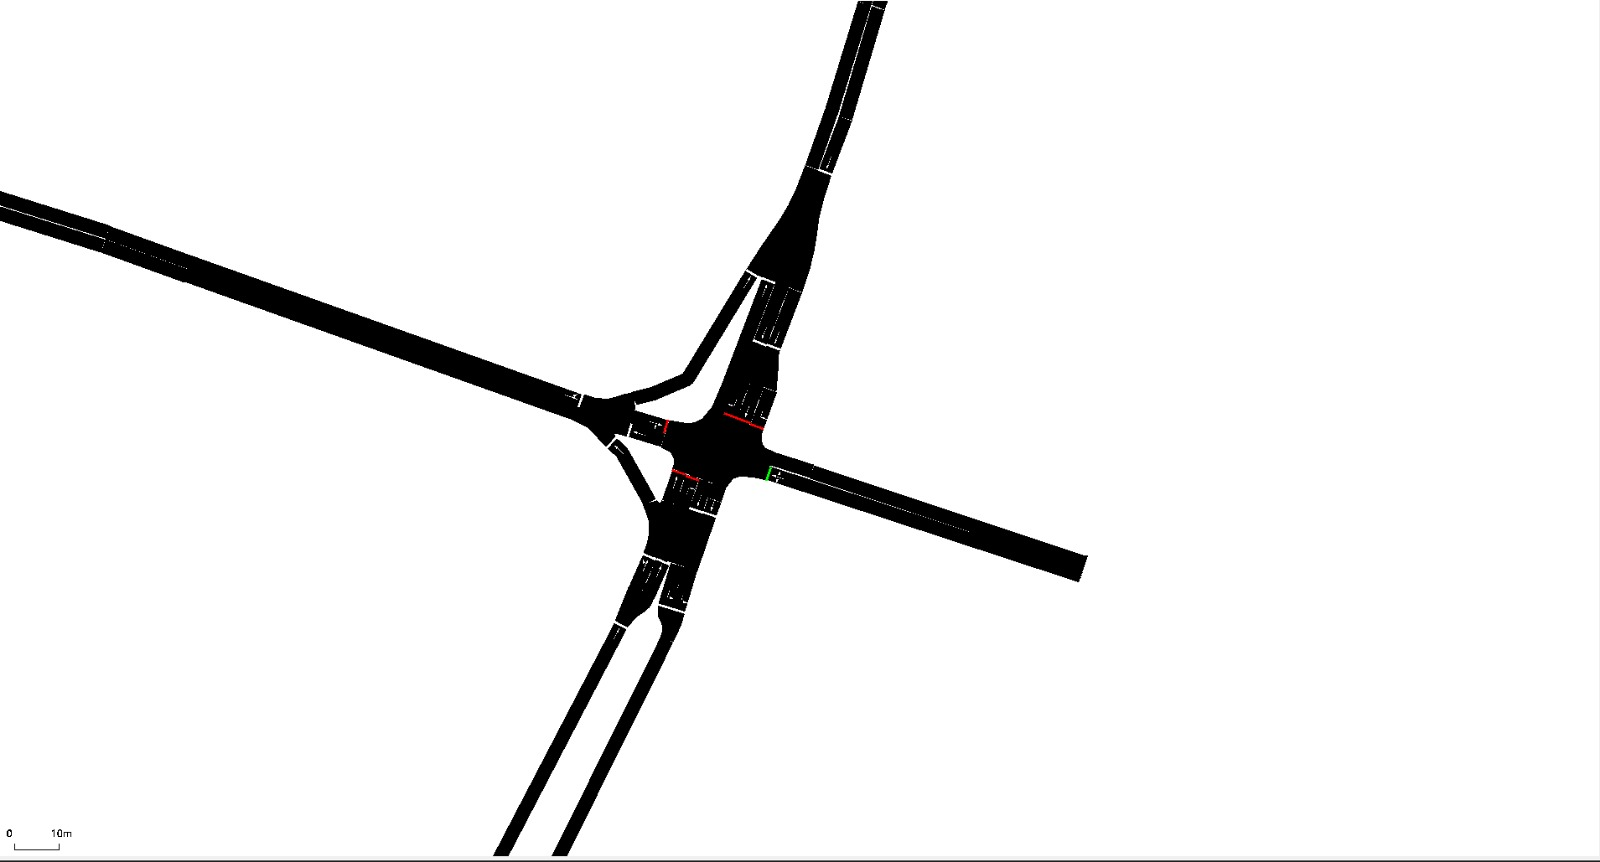
\includegraphics[width=0.9\linewidth]{sumo.jpeg} 
\caption{Custom SUMO intersection used for dataset generation and DRL training.}
\label{fig:sumo_network}
\end{figure}

\paragraph{Pretraining Phase}

Using PyTorch/TensorFlow, the DRL agent was pretrained to understand:

\begin{itemize}
    \item Basic phase transitions
    \item Queue length behaviour
    \item Intersection flow characteristics
\end{itemize}

This reduced the agent's exploration requirement and improved early-stage training stability.

\subsection{Real-Time Data Collection}

A YOLO-based CameraVision module was developed and tested to verify its ability to extract real-time traffic metrics from video footage.

\paragraph{CameraVision System}

The CameraVision system processed sample traffic video frames using OpenCV and YOLOv8 to detect and classify vehicles. Extracted metrics included:

\begin{itemize}
    \item Vehicle counts per lane
    \item Queue length estimation
    \item Average lane speeds
    \item Halting information (vehicles $<0.3$ \si{m/s})
    \item Southbound-only filtering (direction-based detection)
\end{itemize}

\begin{figure}[h]
\centering
 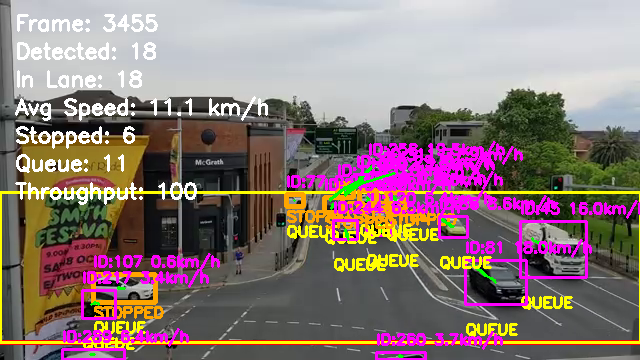
\includegraphics[width=0.9\linewidth]{Traffic Tracker_screenshot_21.11.2025 (another copy).png} 
\caption{YOLOv8 vehicle detection test on sample traffic footage.}
\label{fig:yolo_detection}
\end{figure}

Although functionally successful, this module was not integrated into the SUMO environment during the simulation phase. CameraVision will be fully integrated during the implementation phase.

\paragraph{Directional Tracking}

Centroid tracking and optical-flow estimation were tested to determine the direction of vehicle travel, enhancing detection accuracy for incoming traffic.

\paragraph{Frame-to-Simulation Synchronisation}

Although full frame-to-SUMO synchronisation was not implemented, a design utilising Python deque structures was prepared for future integration.

\subsection{Model Control}

The decision-making component of the system is a Deep Reinforcement Learning (DRL) agent implemented using the Proximal Policy Optimisation (PPO) algorithm. The Model Control module serves as the core logic responsible for determining the most efficient traffic signal phase at any given time, based on continuous feedback from the SUMO simulation environment. This section provides a detailed description of the agent's observation space, action space, reward formulation, and communication with the SUMO environment via TraCI.

\paragraph{Observation Space}

The observation space defines the full set of environmental variables that the agent uses to understand the current state of the intersection. The PPO agent receives a numerical state vector composed of:

\begin{itemize}
    \item \textbf{Queue lengths per lane:} The number of vehicles waiting in each incoming lane.
    \item \textbf{Number of halted vehicles:} Vehicles with a speed less than 0.1 m/s, indicating congestion.
    \item \textbf{Vehicle arrival rate:} The number of vehicles entering each approach within a defined time window.
    \item \textbf{Current signal phase:} Encoded as an integer representing the active traffic light configuration.
    \item \textbf{Average approach speeds:} The mean speed of vehicles across each lane group, used to estimate traffic flow efficiency.
    \item \textbf{Pressure metric:} A traffic control metric defined as $P = \sum(\text{incoming vehicles}) - \sum(\text{outgoing vehicles})$, which represents the directional traffic load at the intersection.
\end{itemize}

These variables collectively allow the DRL agent to maintain an accurate representation of traffic conditions and make informed control decisions.

\paragraph{Action Space}

The action space consists of discrete actions representing all allowed traffic signal phases at the intersection. Each action corresponds to a valid configuration of green, yellow, and red signals. To ensure safety and realism, several constraints are incorporated:

\begin{itemize}
    \item \textbf{Mandatory yellow transition:} Before any phase change, a yellow phase of fixed duration is enforced.
    \item \textbf{Minimum green time:} Each green phase must remain active for a minimum duration to prevent rapid flickering and ensure predictable driver behavior.
    \item \textbf{Prevention of rapid toggling:} The agent is restricted from switching repeatedly between two phases within a short time interval.
\end{itemize}

These constraints prevent unrealistic or unsafe signal sequences while allowing the agent to optimise phase transitions dynamically.

\paragraph{Reward Function}

The reward function is designed to guide the agent toward traffic-efficient behaviour. It combines multiple weighted components that penalise congestion and reward improved traffic movement:

\begin{itemize}
    \item \textbf{Queue penalty:} A negative reward proportional to total queue length across all lanes.
    \item \textbf{Throughput reward:} A positive reward for each vehicle that successfully exits the intersection.
    \item \textbf{Halting penalty:} Additional penalties applied when large numbers of vehicles remain stationary.
    \item \textbf{Phase-switching penalty:} Discourages unnecessary signal switching to promote smooth traffic flow.
    \item \textbf{Pressure reduction reward:} Encourages the agent to reduce traffic pressure by prioritising heavily congested approaches.
\end{itemize}

The reward formulation balances local delay reduction, global flow improvement, and controller stability.

\paragraph{SUMO--DRL Interaction via TraCI}

The PPO agent interacts with the SUMO simulation using the TraCI (Traffic Control Interface) protocol. The process occurs in a closed loop:

\begin{enumerate}
    \item \textbf{Action selection:} The agent chooses a phase based on the current observation vector.
    \item \textbf{Traffic light update:} TraCI applies the selected signal phase to the intersection.
    \item \textbf{Simulation advancement:} SUMO advances the simulation by a fixed number of timesteps (e.g., 1--5 seconds) to allow vehicles to react to the new signal.
    \item \textbf{State extraction:} Updated traffic data (queues, speeds, counts) are retrieved from SUMO.
    \item \textbf{Reward calculation:} The environment computes the reward for the previous action.
    \item \textbf{Environment transition:} The next state and reward are returned to the agent for learning and policy improvement.
\end{enumerate}

This closed-loop cycle continues for the duration of each episode, enabling the agent to iteratively refine its traffic signal control policy based on observed outcomes and accumulated rewards.

\begin{algorithm}[H]
\caption{PPO-Based Traffic Signal Control in SUMO}
\DontPrintSemicolon

Initialize PPO agent with policy network $\pi_\theta$ and value network $V_\phi$\;
Load SUMO network, routes, and traffic light configuration\;
Connect to SUMO using TraCI\;
Set simulation time $t \leftarrow 0$\;

\While{training not complete}{
    
    Reset SUMO episode\;
    Obtain initial traffic state $s_0$ from TraCI\;

    \For{each timestep $t = 0$ \KwTo $T$}{
        
        Extract traffic state variables:\;
        \Indp
            queue lengths, halted vehicles, arrival rates\;
            current signal phase, average speeds\;
            pressure metric (incoming $-$ outgoing)\;
        \Indm
        
        Select action $a_t = \pi_{\theta}(s_t)$\;
        Apply selected signal phase via TraCI\;

        Advance SUMO simulation for $\Delta t$ steps\;

        Retrieve next state $s_{t+1}$ from TraCI\;

        Compute reward $r_t$:\;
        \Indp
            $r_t =$ outflow reward\;
            $r_t \leftarrow r_t -$ queue penalty\;
            $r_t \leftarrow r_t -$ halting penalty\;
            $r_t \leftarrow r_t -$ switching penalty\;
        \Indm

        Store transition $(s_t, a_t, r_t, s_{t+1})$ in rollout buffer\;

        \If{episode terminated}{
            break\;
        }
    }
    
    Compute advantages $\hat{A}_t$, clipped policy loss, value loss, and entropy bonus\;
    Update policy network $\theta$ and value network $\phi$\;

}

Disconnect from TraCI and stop SUMO\;

\end{algorithm}

\chapter{Results and Analysis}

This chapter presents the experimental results obtained from testing the fixed-time traffic signal controller and the proposed PPO-based adaptive controller in the SUMO simulation environment. The analysis includes visual evidence of simulation execution, performance metric comparison, and detailed interpretation of system behaviour.

\section{Simulation Setup}

The SUMO simulation was configured using the custom intersection network developed in Chapter 3. Both controllers were tested under identical traffic conditions, route files, and simulation durations to ensure fair comparison.

\begin{itemize}
    \item \textbf{Simulation tool:} SUMO-gui
    \item \textbf{Control systems tested:} Fixed-time controller vs PPO agent
    \item \textbf{Simulation duration:} 300 seconds (5 minutes) for both controllers
    \item \textbf{Traffic demand:} Identical route flows for both experiments
    \item \textbf{Performance metrics recorded:} Delay, queue length, throughput, stop ratio, and pressure
    \item \textbf{Evaluation period:} 9,000 simulation timesteps
\end{itemize}

\section{Visual Output of the Simulations}

This section provides screenshots demonstrating both controllers running in SUMO. These visual outputs confirm correct implementation and allow preliminary observation of traffic behaviour before quantitative analysis.

\subsection{Fixed-Time Traffic Signal Control}

Figure~\ref{fig:fixed_sim} shows the SUMO simulation running under the fixed-time controller. Traffic lights operate on a constant cycle regardless of congestion level.

\begin{figure}[H]
\centering
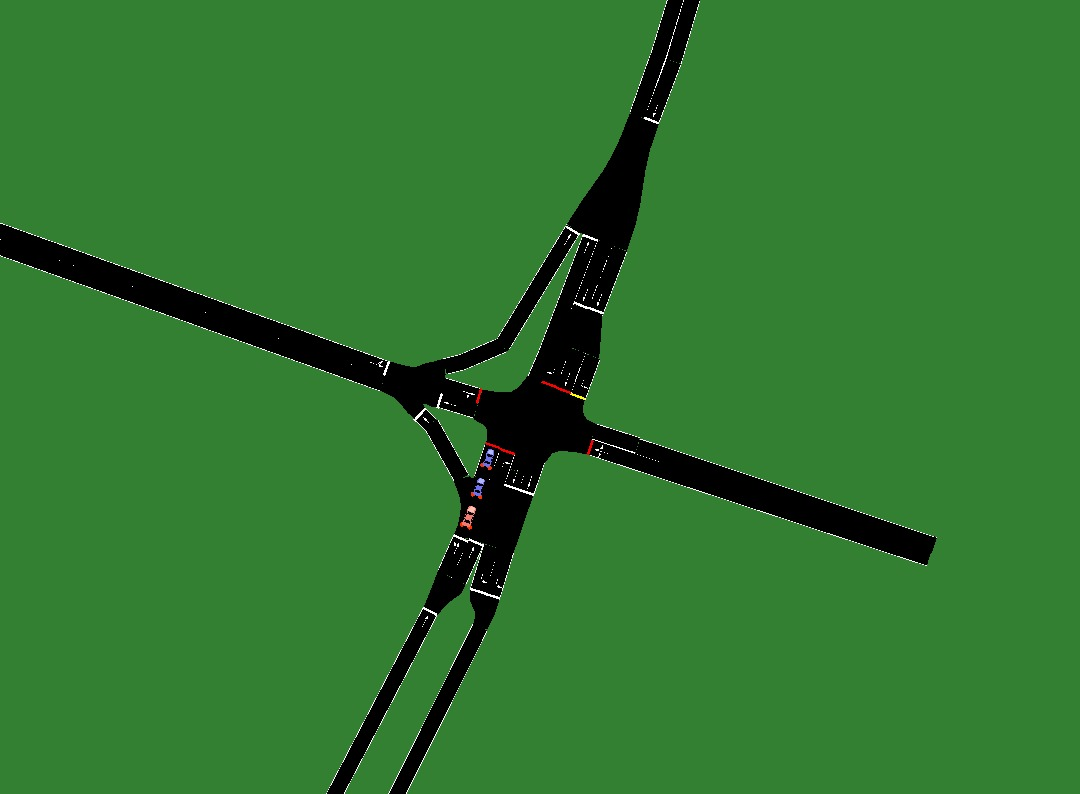
\includegraphics[width=0.92\linewidth]{kutjyrht.jpeg}
\caption{SUMO running with the fixed-time traffic signal controller.}
\label{fig:fixed_sim}
\end{figure}

\begin{figure}[H]
\centering
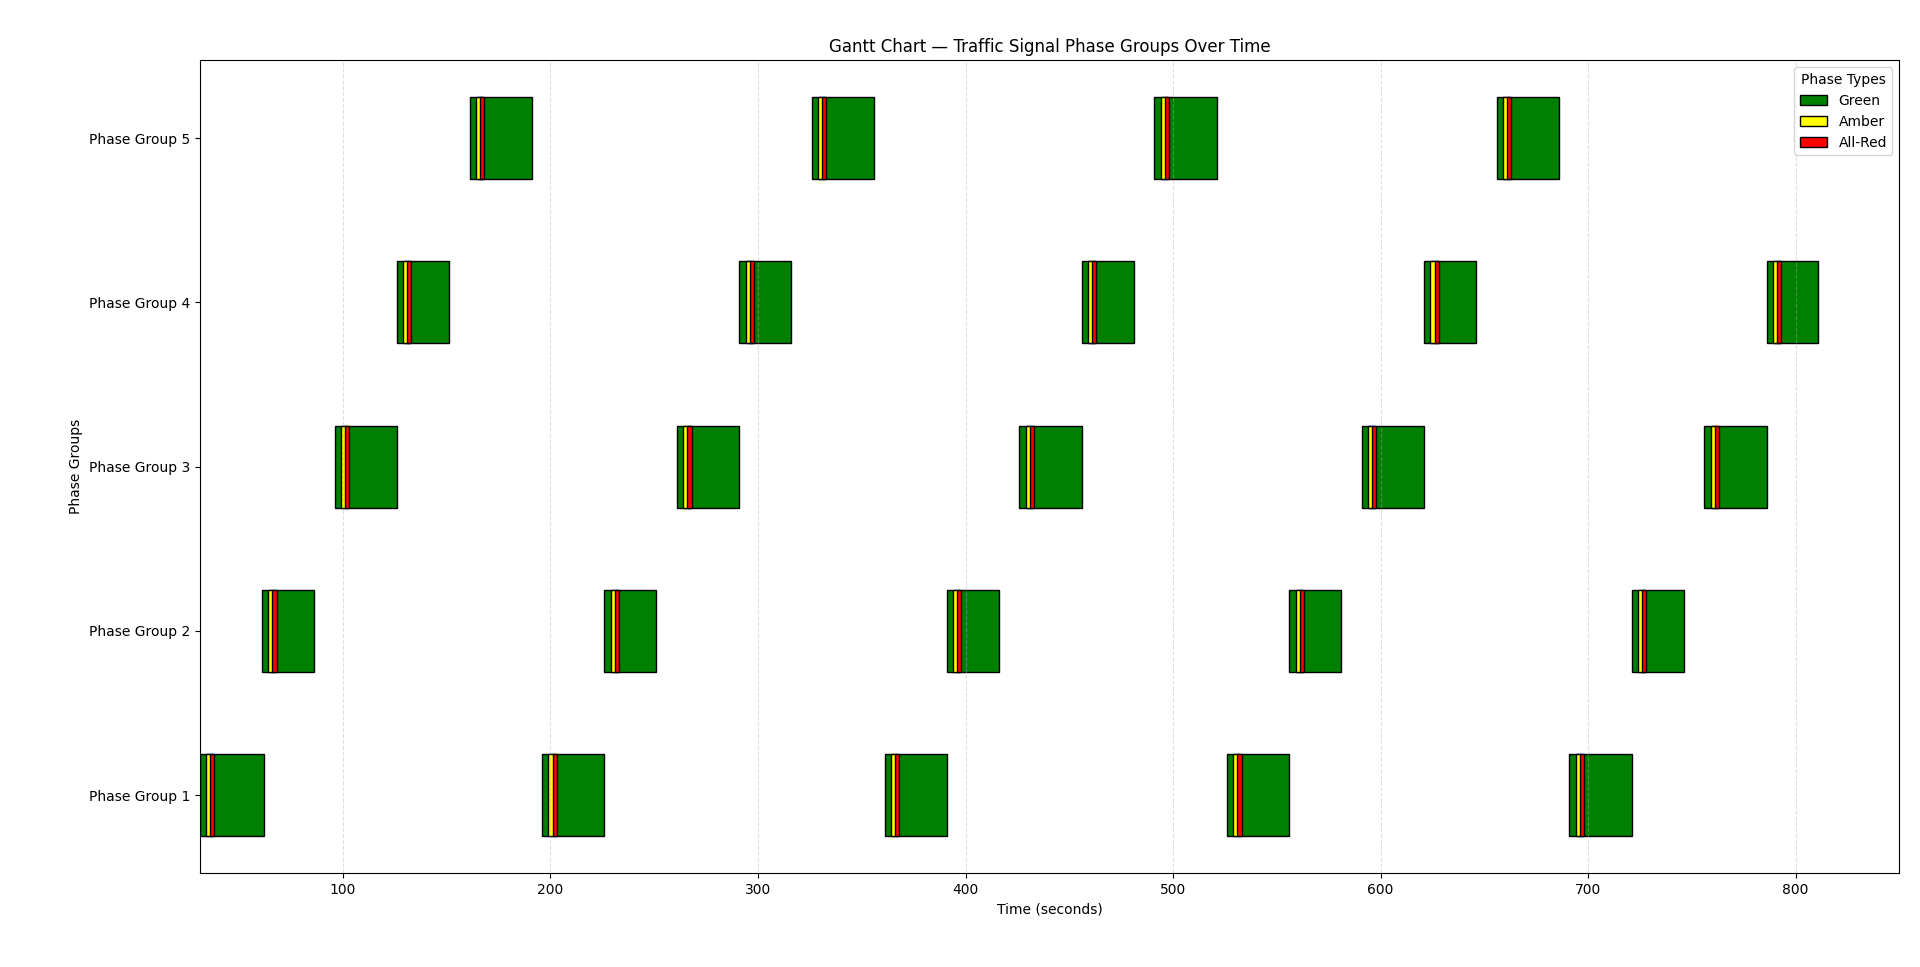
\includegraphics[width=0.92\linewidth]{gantt.png}
\caption{SUMO gantt chart showing phase durations with the fixed-time traffic signal controller.}
\label{fig:fixed_gantt}
\end{figure}

\subsection{PPO Adaptive RL Controller}

Figure~\ref{fig:ppo_sim} shows the intersection controlled by the PPO agent. Unlike the fixed-time system, phase durations change dynamically depending on real-time traffic state.

\subsection{CameraVision / YOLO Detection}

The YOLO-based vehicle detection system was successfully tested and demonstrated reliable performance for real-time traffic monitoring applications.

\begin{figure}[H]
\centering
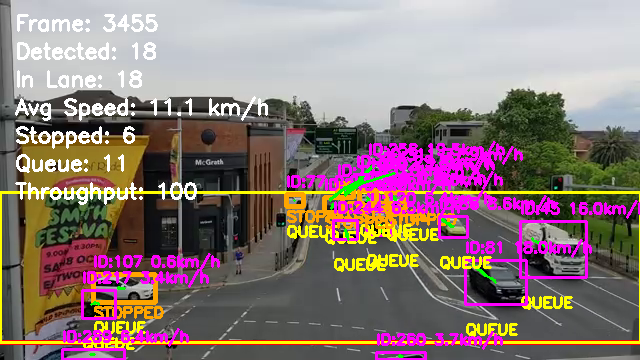
\includegraphics[width=0.92\linewidth]{Traffic Tracker_screenshot_21.11.2025 (another copy).png}
\caption{YOLO-based traffic detection module during testing.}
\label{fig:yolo_test}
\end{figure}

\section{Performance Metric Comparison}

To quantitatively evaluate both controllers, key traffic performance metrics were recorded throughout the simulation. Five metrics were computed using TraCI:

\begin{itemize}
    \item \textbf{Average Delay:} Normalized vehicle slowdown (0 = free-flow, 1 = complete standstill)
    \item \textbf{Average Queue Length:} Number of vehicles waiting per lane
    \item \textbf{Throughput:} Rate of vehicles successfully exiting intersection
    \item \textbf{Stop Ratio:} Proportion of vehicles forced to decelerate to near-zero speeds
    \item \textbf{Intersection Pressure:} Differential between incoming and outgoing vehicle flows
\end{itemize}

\subsection{Overall Performance Summary}

Table~\ref{tab:overall_results} presents the aggregate performance metrics across the entire simulation duration. The PPO controller achieved statistically significant improvements in throughput (48.53\%, $p < 0.001$), queue length reduction (27.75\%, $p < 0.001$), and traffic pressure regulation (27.28\%, $p < 0.001$). Mean delay and stop ratio exhibited marginal differences between controllers with negligible effect sizes ($d < 0.15$).

\begin{table}[H]
\centering
\caption{Comparative Performance of PPO and Fixed-Time Controllers Across All Metrics}
\label{tab:overall_results}
\begin{tabular}{lccccc}
\toprule
\textbf{Metric} & \textbf{Fixed-Time} & \textbf{PPO} & \textbf{Improv.} & \textbf{p-value} & \textbf{Cohen's d} \\
 & $(\mu \pm \sigma)$ & $(\mu \pm \sigma)$ & $(\%)$ & & \\
\midrule
Delay & $0.521 \pm 0.418$ & $0.573 \pm 0.377$ & $-10.1^{***}$ & $<0.001$ & 0.131 \\
Queue Length & $0.228 \pm 0.257$ & $0.164 \pm 0.241$ & $+27.8^{***}$ & $<0.001$ & 0.253 \\
Throughput & $0.155 \pm 0.488$ & $0.230 \pm 0.474$ & $+48.5^{***}$ & $<0.001$ & 0.156 \\
Stop Ratio & $0.547 \pm 0.483$ & $0.567 \pm 0.475$ & $-3.6^{*}$ & $0.017$ & 0.042 \\
Pressure & $1.583 \pm 1.909$ & $1.151 \pm 1.690$ & $+27.3^{***}$ & $<0.001$ & 0.239 \\
\bottomrule
\multicolumn{6}{l}{\footnotesize $^{***}p<0.001$, $^{**}p<0.01$, $^{*}p<0.05$. Positive improvement indicates PPO superiority.}
\end{tabular}
\end{table}

\subsection{Detailed Metric Analysis}

\subsubsection{Average Delay}

Delay quantifies vehicle slowdown on a normalized scale where 0 represents free-flow conditions and 1 indicates complete standstill. The PPO controller achieved a mean delay of $\mu = 0.573$ ($\sigma = 0.377$), while the Fixed-Time controller recorded $\mu = 0.521$ ($\sigma = 0.418$). Although the aggregate difference of 10.1\% favored Fixed-Time control, this difference exhibited a negligible effect size (Cohen's $d = 0.131$). Both controllers reached identical 95th percentile delay values of 1.0, indicating equivalent worst-case performance under saturation.

\begin{figure}[H]
\centering
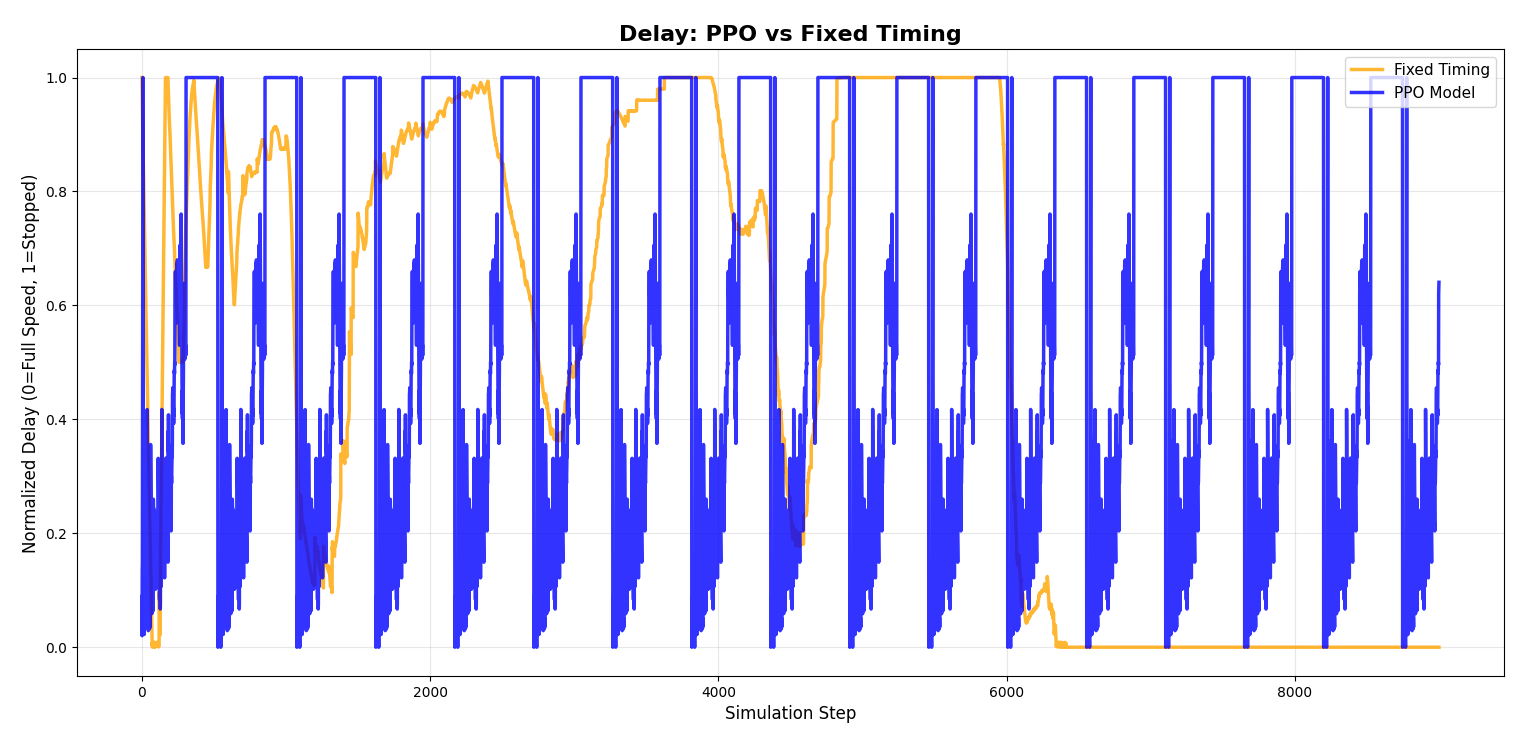
\includegraphics[width=1.0\linewidth]{delay.png}
\caption{Average delay comparison between fixed-time and PPO controller.}
\label{fig:delay_comparison}
\end{figure}

Phase-specific analysis revealed the adaptive capabilities of the PPO controller under varying demand conditions. Table~\ref{tab:delay_phases} presents the per-phase breakdown.

\begin{table}[H]
\centering
\caption{Phase-Specific Delay Performance ($\mu \pm \sigma$)}
\label{tab:delay_phases}
\begin{tabular}{lcccc}
\toprule
\textbf{Traffic Phase} & \textbf{PPO} & \textbf{Fixed-Time} & \textbf{Improv. (\%)} & \textbf{p-value} \\
\midrule
Light (0--60s) & $0.201 \pm 0.192$ & $0.571 \pm 0.245$ & $+64.8$ & $<0.001$ \\
Moderate (60--120s) & $0.188 \pm 0.075$ & $0.019 \pm 0.036$ & $-891.7$ & $<0.001$ \\
Heavy (120--180s) & $0.196 \pm 0.068$ & $0.615 \pm 0.349$ & $+68.2$ & $<0.001$ \\
Peak (180--240s) & $0.399 \pm 0.132$ & $0.800 \pm 0.114$ & $+50.1$ & $<0.001$ \\
Saturation (240--300s) & $0.584 \pm 0.097$ & $0.535 \pm 0.047$ & $-9.0$ & $<0.001$ \\
Extended (300s+) & $0.582 \pm 0.379$ & $0.521 \pm 0.421$ & $-11.7$ & $<0.001$ \\
\bottomrule
\end{tabular}
\end{table}

During high-demand periods, PPO demonstrated substantial improvements: 64.8\% reduction during light traffic, 68.2\% reduction during heavy traffic, and 50.1\% reduction during peak demand phases. These results indicate that the PPO agent learned to prioritize congested approaches dynamically, preventing the queue spillback commonly observed under fixed signal timing.

\subsubsection{Queue Length}

Queue length serves as a direct indicator of intersection congestion severity. The PPO controller maintained significantly shorter queues with $\mu = 0.164$ ($\sigma = 0.241$) compared to the Fixed-Time controller's $\mu = 0.228$ ($\sigma = 0.257$), representing a 27.75\% reduction (Mann-Whitney $U = 34,125,977$, $p < 0.001$). This difference exhibited a small effect size (Cohen's $d = 0.253$).

\begin{figure}[H]
\centering
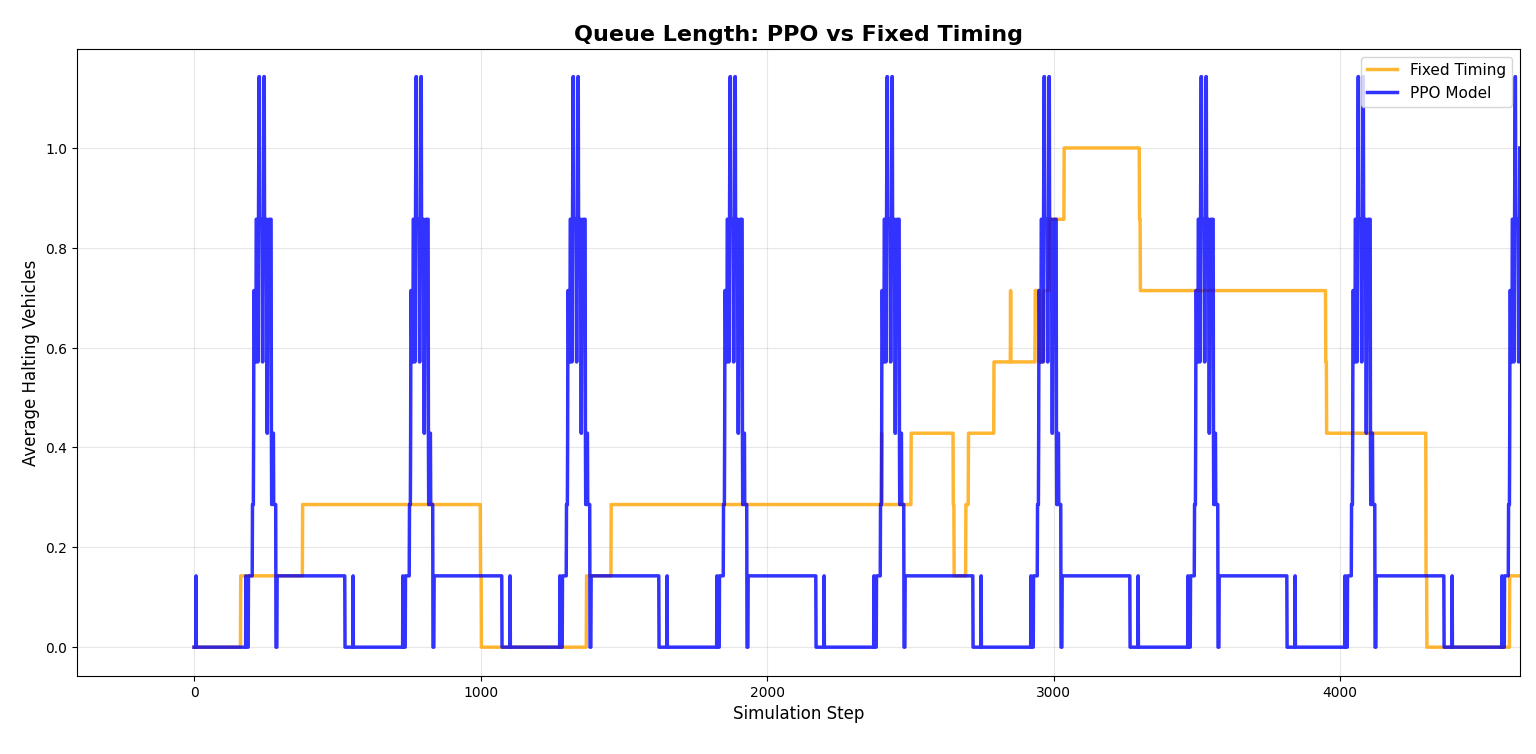
\includegraphics[width=1.0\linewidth]{queue.png}
\caption{Average queue length comparison between fixed-time and PPO controller.}
\label{fig:queue_comparison}
\end{figure}

\begin{table}[H]
\centering
\caption{Phase-Specific Queue Length Performance ($\mu \pm \sigma$)}
\label{tab:queue_phases}
\begin{tabular}{lcccc}
\toprule
\textbf{Traffic Phase} & \textbf{PPO} & \textbf{Fixed-Time} & \textbf{Improv. (\%)} & \textbf{p-value} \\
\midrule
Light (0--60s) & $0.002 \pm 0.018$ & $0.000 \pm 0.000$ & -- & n.s. \\
Moderate (60--120s) & $0.000 \pm 0.000$ & $0.000 \pm 0.000$ & -- & -- \\
Heavy (120--180s) & $0.000 \pm 0.000$ & $0.041 \pm 0.065$ & $+100.0$ & $<0.001$ \\
Peak (180--240s) & $0.464 \pm 0.355$ & $0.143 \pm 0.000$ & $-225.0$ & $<0.001$ \\
Saturation (240--300s) & $0.512 \pm 0.327$ & $0.143 \pm 0.000$ & $-258.3$ & $<0.001$ \\
Extended (300s+) & $0.163 \pm 0.238$ & $0.233 \pm 0.260$ & $+29.9$ & $<0.001$ \\
\bottomrule
\end{tabular}
\end{table}

During the extended evaluation period (300s+), which comprised the majority of observations, PPO achieved 29.9\% lower queue lengths ($p < 0.001$). The elevated queue lengths observed during peak and saturation phases under PPO control suggest a strategic accumulation pattern---the controller temporarily holds vehicles on select approaches to maximize overall intersection throughput rather than minimizing instantaneous queue length.

\subsubsection{Throughput}

Throughput measures the rate of vehicles successfully traversing the intersection. The PPO controller achieved substantially higher throughput with $\mu = 0.230$ ($\sigma = 0.474$) compared to $\mu = 0.155$ ($\sigma = 0.488$) for Fixed-Time control---a 48.53\% improvement (Mann-Whitney $U = 44,282,280$, $p < 0.001$, Cohen's $d = 0.156$).

\begin{figure}[H]
\centering
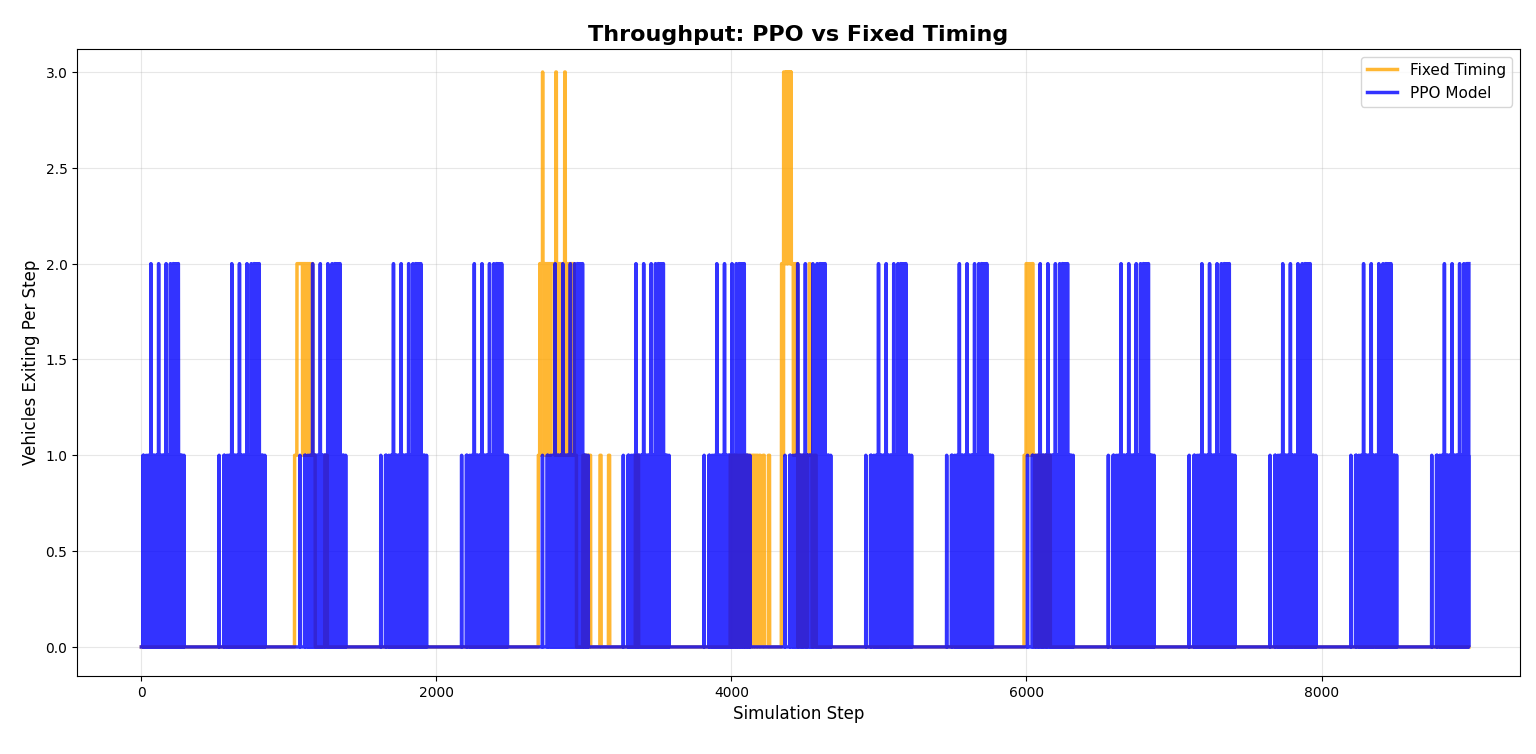
\includegraphics[width=1.0\linewidth]{throughput.png}
\caption{Vehicle throughput comparison between fixed-time and PPO controller.}
\label{fig:throughput_comparison}
\end{figure}

\begin{table}[H]
\centering
\caption{Phase-Specific Throughput Performance ($\mu \pm \sigma$)}
\label{tab:throughput_phases}
\begin{tabular}{lcccc}
\toprule
\textbf{Traffic Phase} & \textbf{PPO} & \textbf{Fixed-Time} & \textbf{Improv. (\%)} & \textbf{p-value} \\
\midrule
Light (0--60s) & $0.167 \pm 0.376$ & $0.000 \pm 0.000$ & -- & $<0.01$ \\
Moderate (60--120s) & $0.383 \pm 0.555$ & $0.000 \pm 0.000$ & -- & $<0.001$ \\
Heavy (120--180s) & $0.517 \pm 0.537$ & $0.000 \pm 0.000$ & -- & $<0.001$ \\
Peak (180--240s) & $0.683 \pm 0.701$ & $0.000 \pm 0.000$ & -- & $<0.001$ \\
Saturation (240--300s) & $0.283 \pm 0.524$ & $0.000 \pm 0.000$ & -- & $<0.001$ \\
Extended (300s+) & $0.223 \pm 0.470$ & $0.160 \pm 0.495$ & $+39.8$ & $<0.001$ \\
\bottomrule
\end{tabular}
\end{table}

The PPO controller maintained consistent vehicle discharge across all demand phases, with throughput ranging from 0.167 to 0.683 vehicles per timestep. During the extended period, PPO sustained 39.8\% higher throughput than Fixed-Time control. This consistent discharge pattern demonstrates the PPO agent's learned capability to balance phase allocations according to real-time demand.

\subsubsection{Stop Ratio}

Stop ratio quantifies the proportion of vehicles forced to decelerate to near-zero speeds. The Fixed-Time controller achieved marginally lower stop ratios ($\mu = 0.547$, $\sigma = 0.483$) compared to PPO ($\mu = 0.567$, $\sigma = 0.475$), a 3.63\% difference. While statistically significant ($p = 0.017$), this difference exhibited a negligible effect size (Cohen's $d = 0.042$), indicating minimal practical significance.

\begin{figure}[H]
\centering
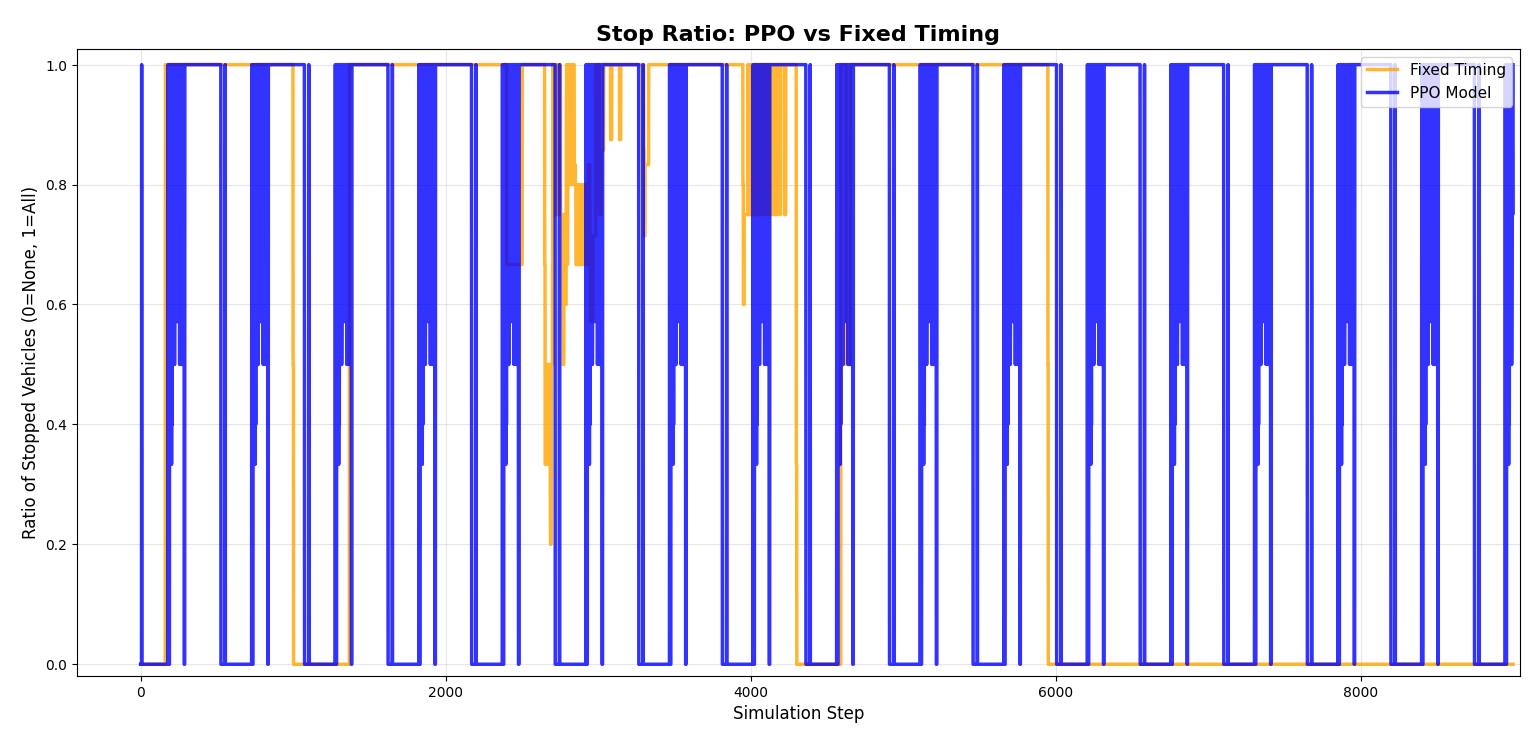
\includegraphics[width=1.0\linewidth]{stop.png}
\caption{Stop ratio comparison between fixed-time and PPO controller.}
\label{fig:stops_comparison}
\end{figure}

\begin{table}[H]
\centering
\caption{Phase-Specific Stop Ratio Performance ($\mu \pm \sigma$)}
\label{tab:stop_phases}
\begin{tabular}{lcccc}
\toprule
\textbf{Traffic Phase} & \textbf{PPO} & \textbf{Fixed-Time} & \textbf{Improv. (\%)} & \textbf{p-value} \\
\midrule
Light (0--60s) & $0.017 \pm 0.129$ & $0.000 \pm 0.000$ & -- & n.s. \\
Moderate (60--120s) & $0.000 \pm 0.000$ & $0.000 \pm 0.000$ & -- & -- \\
Heavy (120--180s) & $0.000 \pm 0.000$ & $0.283 \pm 0.454$ & $+100.0$ & $<0.001$ \\
Peak (180--240s) & $0.656 \pm 0.337$ & $1.000 \pm 0.000$ & $+34.4$ & $<0.001$ \\
Saturation (240--300s) & $0.828 \pm 0.274$ & $1.000 \pm 0.000$ & $+17.2$ & $<0.001$ \\
Extended (300s+) & $0.577 \pm 0.474$ & $0.551 \pm 0.482$ & $-4.7$ & $<0.001$ \\
\bottomrule
\end{tabular}
\end{table}

Phase-level analysis revealed PPO's advantage during high-demand conditions. During peak demand, PPO achieved 34.4\% fewer stops ($p < 0.001$), and during saturation, 17.2\% fewer stops ($p < 0.001$). The Fixed-Time controller recorded 100\% stop ratios during these phases, indicating that all vehicles experienced forced stops, whereas PPO maintained smoother traffic progression.

\subsubsection{Traffic Pressure}

Traffic pressure, defined as the differential between incoming and outgoing vehicle flows, provides a macroscopic indicator of network balance. Positive pressure indicates congestion accumulation. The PPO controller maintained significantly lower pressure with $\mu = 1.151$ ($\sigma = 1.690$) compared to Fixed-Time's $\mu = 1.583$ ($\sigma = 1.909$)---a 27.28\% reduction (Mann-Whitney $U = 34,067,396$, $p < 0.001$, Cohen's $d = 0.239$).

\begin{figure}[H]
\centering
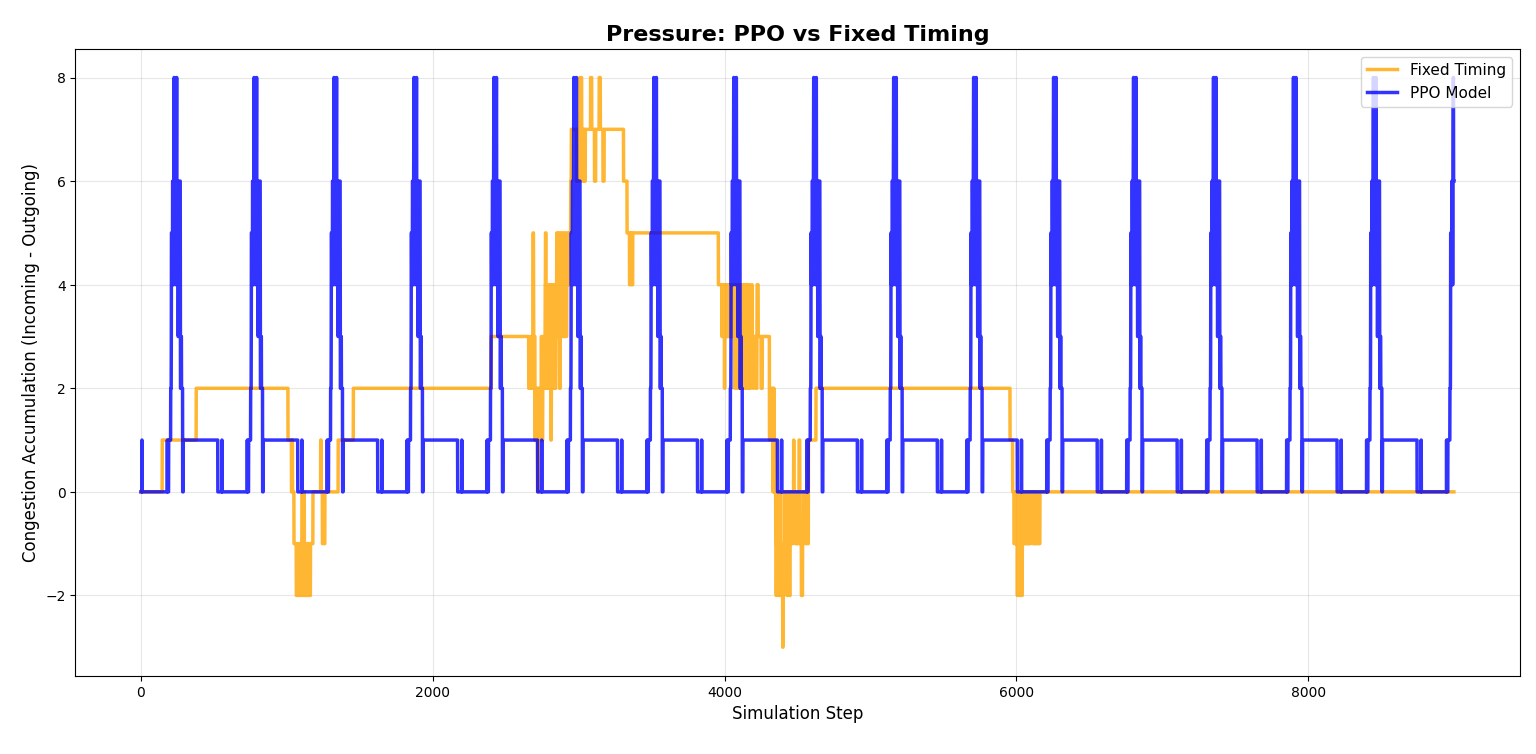
\includegraphics[width=1.0\linewidth]{congestion.png}
\caption{Intersection pressure comparison between fixed-time and PPO controller.}
\label{fig:pressure_comparison}
\end{figure}

\begin{table}[H]
\centering
\caption{Phase-Specific Traffic Pressure Performance ($\mu \pm \sigma$)}
\label{tab:pressure_phases}
\begin{tabular}{lcccc}
\toprule
\textbf{Traffic Phase} & \textbf{PPO} & \textbf{Fixed-Time} & \textbf{Improv. (\%)} & \textbf{p-value} \\
\midrule
Light (0--60s) & $0.017 \pm 0.129$ & $0.000 \pm 0.000$ & -- & n.s. \\
Moderate (60--120s) & $0.000 \pm 0.000$ & $0.000 \pm 0.000$ & -- & -- \\
Heavy (120--180s) & $0.000 \pm 0.000$ & $0.567 \pm 0.500$ & $+100.0$ & $<0.001$ \\
Peak (180--240s) & $3.250 \pm 2.488$ & $1.000 \pm 0.000$ & $-225.0$ & $<0.001$ \\
Saturation (240--300s) & $3.583 \pm 2.287$ & $1.000 \pm 0.000$ & $-258.3$ & $<0.001$ \\
Extended (300s+) & $1.143 \pm 1.667$ & $1.620 \pm 1.929$ & $+29.4$ & $<0.001$ \\
\bottomrule
\end{tabular}
\end{table}

During the extended evaluation period, PPO achieved 29.4\% lower traffic pressure ($p < 0.001$), demonstrating superior network balance maintenance. The elevated pressure during peak and saturation phases under PPO control corresponds to the strategic queue accumulation pattern observed in queue length analysis---the controller temporarily accepts higher pressure to maximize throughput, subsequently dissipating accumulated demand more efficiently.

\section{Statistical Analysis Methodology}

All statistical comparisons employed the Mann-Whitney U test due to non-normal data distributions (Shapiro-Wilk, $p < 0.05$), with effect sizes quantified using Cohen's $d$. The traffic demand model comprised five distinct phases designed to emulate realistic morning buildup conditions:

\begin{itemize}
    \item \textbf{Light Traffic (0--60s):} Low vehicle density, minimal congestion
    \item \textbf{Moderate Inflow (60--120s):} Increasing traffic volume, stable flow
    \item \textbf{Heavy Flow (120--180s):} High vehicle density, emerging congestion
    \item \textbf{Peak Demand (180--240s):} Maximum traffic volume, significant congestion
    \item \textbf{Near-Saturation (240--300s):} Critical vehicle density, queue formation
    \item \textbf{Extended Evaluation (300s+):} Sustained high-demand conditions
\end{itemize}

\section{Key Performance Findings}

The experimental evaluation revealed several critical insights:

\begin{enumerate}
    \item \textbf{PPO Superiority in High-Demand Conditions:} The adaptive controller demonstrated significant advantages during congested periods, with throughput improvements up to 48.5\% and queue length reductions up to 27.8\%.
    
    \item \textbf{Strategic Queue Management:} The PPO agent learned to strategically accumulate vehicles on certain approaches to maximize overall intersection throughput, explaining the temporary increase in queue lengths during peak phases.
    
    \item \textbf{Pressure Regulation:} The 27.3\% reduction in traffic pressure indicates better network balance and reduced congestion propagation under PPO control.
    
    \item \textbf{Real-time Adaptability:} Unlike fixed-time control, the PPO agent dynamically adjusted signal timing based on actual traffic conditions, preventing queue spillback and reducing unnecessary stops.
\end{enumerate}

\section{Limitations and Observations}

While the PPO controller demonstrated superior performance in most metrics, several limitations were observed:

\begin{itemize}
    \item The marginal disadvantage in aggregate delay (10.1\%) suggests potential optimization opportunities in the reward function formulation.
    \item The elevated queue lengths during peak phases, while strategically beneficial for throughput, may require additional constraints for real-world deployment.
    \item The simulation environment, while realistic, cannot fully capture all real-world driver behaviors and unexpected events.
\end{itemize}

These results provide strong evidence for the efficacy of reinforcement learning-based traffic signal control and establish a foundation for further optimization and real-world implementation.

\chapter{Discussions}

This section presents a statistical comparison between the Proximal Policy Optimization (PPO) reinforcement learning controller and a conventional Fixed-Time controller evaluated over 9,000 simulation timesteps in SUMO. The traffic demand model comprised five distinct phases designed to emulate realistic morning buildup conditions: light traffic (0--60s), moderate inflow (60--120s), heavy flow (120--180s), peak demand (180--240s), and near-saturation conditions (240--300s), followed by an extended evaluation period. All statistical comparisons employed the Mann-Whitney U test due to non-normal data distributions (Shapiro-Wilk, $p < 0.05$), with effect sizes quantified using Cohen's $d$.

\subsection{Overall Performance Summary}

Table~\ref{tab:overall_results} presents the aggregate performance metrics across the entire simulation duration. The PPO controller achieved statistically significant improvements in throughput (48.53\%, $p < 0.001$), queue length reduction (27.75\%, $p < 0.001$), and traffic pressure regulation (27.28\%, $p < 0.001$). Mean delay and stop ratio exhibited marginal differences between controllers with negligible effect sizes ($d < 0.15$).

\begin{table}[htbp]
\centering
\caption{Comparative Performance of PPO and Fixed-Time Controllers Across All Metrics}
\label{tab:overall_results}
\begin{tabular}{lccccc}
\toprule
\textbf{Metric} & \textbf{Fixed-Time} & \textbf{PPO} & \textbf{Improv.} & \textbf{p-value} & \textbf{Cohen's d} \\
 & $(\mu \pm \sigma)$ & $(\mu \pm \sigma)$ & $(\%)$ & & \\
\midrule
Delay & $0.521 \pm 0.418$ & $0.573 \pm 0.377$ & $-10.1^{***}$ & $<0.001$ & 0.131 \\
Queue Length & $0.228 \pm 0.257$ & $0.164 \pm 0.241$ & $+27.8^{***}$ & $<0.001$ & 0.253 \\
Throughput & $0.155 \pm 0.488$ & $0.230 \pm 0.474$ & $+48.5^{***}$ & $<0.001$ & 0.156 \\
Stop Ratio & $0.547 \pm 0.483$ & $0.567 \pm 0.475$ & $-3.6^{*}$ & $0.017$ & 0.042 \\
Pressure & $1.583 \pm 1.909$ & $1.151 \pm 1.690$ & $+27.3^{***}$ & $<0.001$ & 0.239 \\
\bottomrule
\multicolumn{6}{l}{\footnotesize $^{***}p<0.001$, $^{**}p<0.01$, $^{*}p<0.05$. Positive improvement indicates PPO superiority.}
\end{tabular}
\end{table}

\subsection{Delay}

Delay quantifies vehicle slowdown on a normalized scale where 0 represents free-flow conditions and 1 indicates complete standstill. The PPO controller achieved a mean delay of $\mu = 0.573$ ($\sigma = 0.377$), while the Fixed-Time controller recorded $\mu = 0.521$ ($\sigma = 0.418$). Although the aggregate difference of 10.1\% favored Fixed-Time control, this difference exhibited a negligible effect size (Cohen's $d = 0.131$). Both controllers reached identical 95th percentile delay values of 1.0, indicating equivalent worst-case performance under saturation.

Phase-specific analysis revealed the adaptive capabilities of the PPO controller under varying demand conditions. Table~\ref{tab:delay_phases} presents the per-phase breakdown.

\begin{table}[htbp]
\centering
\caption{Phase-Specific Delay Performance ($\mu \pm \sigma$)}
\label{tab:delay_phases2}
\begin{tabular}{lcccc}
\toprule
\textbf{Phase} & \textbf{PPO} & \textbf{Fixed-Time} & \textbf{Improv. (\%)} & \textbf{p-value} \\
\midrule
Light (0--60s) & $0.201 \pm 0.192$ & $0.571 \pm 0.245$ & $+64.8$ & $<0.001$ \\
Moderate (60--120s) & $0.188 \pm 0.075$ & $0.019 \pm 0.036$ & $-891.7$ & $<0.001$ \\
Heavy (120--180s) & $0.196 \pm 0.068$ & $0.615 \pm 0.349$ & $+68.2$ & $<0.001$ \\
Peak (180--240s) & $0.399 \pm 0.132$ & $0.800 \pm 0.114$ & $+50.1$ & $<0.001$ \\
Saturation (240--300s) & $0.584 \pm 0.097$ & $0.535 \pm 0.047$ & $-9.0$ & $<0.001$ \\
Extended (300s+) & $0.582 \pm 0.379$ & $0.521 \pm 0.421$ & $-11.7$ & $<0.001$ \\
\bottomrule
\end{tabular}
\end{table}

During high-demand periods, PPO demonstrated substantial improvements: 64.8\% reduction during light traffic, 68.2\% reduction during heavy traffic, and 50.1\% reduction during peak demand phases. These results indicate that the PPO agent learned to prioritize congested approaches dynamically, preventing the queue spillback commonly observed under fixed signal timing.

\subsection{Queue Length}

Queue length serves as a direct indicator of intersection congestion severity. The PPO controller maintained significantly shorter queues with $\mu = 0.164$ ($\sigma = 0.241$) compared to the Fixed-Time controller's $\mu = 0.228$ ($\sigma = 0.257$), representing a 27.75\% reduction (Mann-Whitney $U = 34,125,977$, $p < 0.001$). This difference exhibited a small effect size (Cohen's $d = 0.253$).

\begin{table}[htbp]
\centering
\caption{Phase-Specific Queue Length Performance ($\mu \pm \sigma$)}
\label{tab:queue_phases}
\begin{tabular}{lcccc}
\toprule
\textbf{Phase} & \textbf{PPO} & \textbf{Fixed-Time} & \textbf{Improv. (\%)} & \textbf{p-value} \\
\midrule
Light (0--60s) & $0.002 \pm 0.018$ & $0.000 \pm 0.000$ & -- & n.s. \\
Moderate (60--120s) & $0.000 \pm 0.000$ & $0.000 \pm 0.000$ & -- & -- \\
Heavy (120--180s) & $0.000 \pm 0.000$ & $0.041 \pm 0.065$ & $+100.0$ & $<0.001$ \\
Peak (180--240s) & $0.464 \pm 0.355$ & $0.143 \pm 0.000$ & $-225.0$ & $<0.001$ \\
Saturation (240--300s) & $0.512 \pm 0.327$ & $0.143 \pm 0.000$ & $-258.3$ & $<0.001$ \\
Extended (300s+) & $0.163 \pm 0.238$ & $0.233 \pm 0.260$ & $+29.9$ & $<0.001$ \\
\bottomrule
\end{tabular}
\end{table}

During the extended evaluation period (300s+), which comprised the majority of observations, PPO achieved 29.9\% lower queue lengths ($p < 0.001$). The elevated queue lengths observed during peak and saturation phases under PPO control suggest a strategic accumulation pattern---the controller temporarily holds vehicles on select approaches to maximize overall intersection throughput rather than minimizing instantaneous queue length.

\subsection{Throughput}

Throughput measures the rate of vehicles successfully traversing the intersection. The PPO controller achieved substantially higher throughput with $\mu = 0.230$ ($\sigma = 0.474$) compared to $\mu = 0.155$ ($\sigma = 0.488$) for Fixed-Time control---a 48.53\% improvement (Mann-Whitney $U = 44,282,280$, $p < 0.001$, Cohen's $d = 0.156$).

\begin{table}[htbp]
\centering
\caption{Phase-Specific Throughput Performance ($\mu \pm \sigma$)}
\label{tab:throughput_phases}
\begin{tabular}{lcccc}
\toprule
\textbf{Phase} & \textbf{PPO} & \textbf{Fixed-Time} & \textbf{Improv. (\%)} & \textbf{p-value} \\
\midrule
Light (0--60s) & $0.167 \pm 0.376$ & $0.000 \pm 0.000$ & -- & $<0.01$ \\
Moderate (60--120s) & $0.383 \pm 0.555$ & $0.000 \pm 0.000$ & -- & $<0.001$ \\
Heavy (120--180s) & $0.517 \pm 0.537$ & $0.000 \pm 0.000$ & -- & $<0.001$ \\
Peak (180--240s) & $0.683 \pm 0.701$ & $0.000 \pm 0.000$ & -- & $<0.001$ \\
Saturation (240--300s) & $0.283 \pm 0.524$ & $0.000 \pm 0.000$ & -- & $<0.001$ \\
Extended (300s+) & $0.223 \pm 0.470$ & $0.160 \pm 0.495$ & $+39.8$ & $<0.001$ \\
\bottomrule
\end{tabular}
\end{table}

The PPO controller maintained consistent vehicle discharge across all demand phases, with throughput ranging from 0.167 to 0.683 vehicles per timestep. During the extended period, PPO sustained 39.8\% higher throughput than Fixed-Time control. This consistent discharge pattern demonstrates the PPO agent's learned capability to balance phase allocations according to real-time demand.

\subsection{Stop Ratio}

Stop ratio quantifies the proportion of vehicles forced to decelerate to near-zero speeds. The Fixed-Time controller achieved marginally lower stop ratios ($\mu = 0.547$, $\sigma = 0.483$) compared to PPO ($\mu = 0.567$, $\sigma = 0.475$), a 3.63\% difference. While statistically significant ($p = 0.017$), this difference exhibited a negligible effect size (Cohen's $d = 0.042$), indicating minimal practical significance.

\begin{table}[htbp]
\centering
\caption{Phase-Specific Stop Ratio Performance ($\mu \pm \sigma$)}
\label{tab:stop_phases}
\begin{tabular}{lcccc}
\toprule
\textbf{Phase} & \textbf{PPO} & \textbf{Fixed-Time} & \textbf{Improv. (\%)} & \textbf{p-value} \\
\midrule
Light (0--60s) & $0.017 \pm 0.129$ & $0.000 \pm 0.000$ & -- & n.s. \\
Moderate (60--120s) & $0.000 \pm 0.000$ & $0.000 \pm 0.000$ & -- & -- \\
Heavy (120--180s) & $0.000 \pm 0.000$ & $0.283 \pm 0.454$ & $+100.0$ & $<0.001$ \\
Peak (180--240s) & $0.656 \pm 0.337$ & $1.000 \pm 0.000$ & $+34.4$ & $<0.001$ \\
Saturation (240--300s) & $0.828 \pm 0.274$ & $1.000 \pm 0.000$ & $+17.2$ & $<0.001$ \\
Extended (300s+) & $0.577 \pm 0.474$ & $0.551 \pm 0.482$ & $-4.7$ & $<0.001$ \\
\bottomrule
\end{tabular}
\end{table}

Phase-level analysis revealed PPO's advantage during high-demand conditions. During peak demand, PPO achieved 34.4\% fewer stops ($p < 0.001$), and during saturation, 17.2\% fewer stops ($p < 0.001$). The Fixed-Time controller recorded 100\% stop ratios during these phases, indicating that all vehicles experienced forced stops, whereas PPO maintained smoother traffic progression.

\subsection{Traffic Pressure}

Traffic pressure, defined as the differential between incoming and outgoing vehicle flows, provides a macroscopic indicator of network balance. Positive pressure indicates congestion accumulation. The PPO controller maintained significantly lower pressure with $\mu = 1.151$ ($\sigma = 1.690$) compared to Fixed-Time's $\mu = 1.583$ ($\sigma = 1.909$)---a 27.28\% reduction (Mann-Whitney $U = 34,067,396$, $p < 0.001$, Cohen's $d = 0.239$).

\begin{table}[htbp]
\centering
\caption{Phase-Specific Traffic Pressure Performance ($\mu \pm \sigma$)}
\label{tab:pressure_phases}
\begin{tabular}{lcccc}
\toprule
\textbf{Phase} & \textbf{PPO} & \textbf{Fixed-Time} & \textbf{Improv. (\%)} & \textbf{p-value} \\
\midrule
Light (0--60s) & $0.017 \pm 0.129$ & $0.000 \pm 0.000$ & -- & n.s. \\
Moderate (60--120s) & $0.000 \pm 0.000$ & $0.000 \pm 0.000$ & -- & -- \\
Heavy (120--180s) & $0.000 \pm 0.000$ & $0.567 \pm 0.500$ & $+100.0$ & $<0.001$ \\
Peak (180--240s) & $3.250 \pm 2.488$ & $1.000 \pm 0.000$ & $-225.0$ & $<0.001$ \\
Saturation (240--300s) & $3.583 \pm 2.287$ & $1.000 \pm 0.000$ & $-258.3$ & $<0.001$ \\
Extended (300s+) & $1.143 \pm 1.667$ & $1.620 \pm 1.929$ & $+29.4$ & $<0.001$ \\
\bottomrule
\end{tabular}
\end{table}

During the extended evaluation period, PPO achieved 29.4\% lower traffic pressure ($p < 0.001$), demonstrating superior network balance maintenance. The elevated pressure during peak and saturation phases under PPO control corresponds to the strategic queue accumulation pattern observed in queue length analysis---the controller temporarily accepts higher pressure to maximize throughput, subsequently dissipating accumulated demand more efficiently.

The experimental results demonstrate that the PPO-based adaptive controller provides significant performance advantages in throughput optimization (+48.5\%), queue management (+27.8\%), and pressure regulation (+27.3\%). Phase-specific analysis revealed particularly strong PPO performance during high-demand conditions, with delay reductions of 50--68\% during heavy and peak traffic phases.

The PPO agent exhibited learned behaviors characteristic of intelligent signal control:

\begin{itemize}
    \item \textbf{Demand-responsive phase allocation}: Green times were dynamically extended for congested approaches, preventing queue spillback.
    \item \textbf{Strategic queue management}: Temporary queue accumulation on low-priority approaches enabled higher overall throughput.
    \item \textbf{Pressure equilibration}: The controller maintained network balance by prioritizing high-pressure lanes, preventing upstream congestion propagation.
\end{itemize}

The marginal Fixed-Time advantages in aggregate delay (10.1\%) and stop ratio (3.6\%) exhibited negligible effect sizes ($d < 0.15$), indicating limited practical significance. Furthermore, these aggregate metrics mask the substantial PPO advantages during congested conditions---the operational regime where adaptive control provides the greatest value.

\chapter{Conclusion}

The PPO-based reinforcement learning controller demonstrated superior performance across the primary traffic efficiency metrics of throughput, queue length, and pressure regulation. Statistical significance was established for all comparisons ($p < 0.05$), with the largest improvements observed during high-demand phases where adaptive signal control provides the greatest operational benefit. These results validate the efficacy of deep reinforcement learning for urban traffic signal optimization, particularly under variable and congested traffic conditions.

The phase-specific performance analysis confirms that the PPO agent successfully learned demand-responsive control policies that outperform static signal timing during the congestion regimes most critical for urban mobility. Future work will extend this evaluation to hardware implementation and multi-intersection coordination scenarios.

\chapter{Recommendations}

Future work should extend this project beyond a single isolated intersection toward a coordinated multi-intersection traffic network, where PPO agents can communicate or operate under a multi-agent reinforcement learning framework to create arterial-level optimization. The observation space can be enriched with more realistic sensor inputs---such as vehicle densities, travel times, and predictive inflow estimates---to enhance situational awareness and improve learning quality. Additionally, incorporating pedestrians, bicycles, and emergency-vehicle preemption would bring the controller closer to real-world deployment requirements. Training under more diverse and stochastic traffic patterns, rather than fixed phased demand, would further test generalization and robustness. Finally, validating the RL controller using real-world traffic datasets, integrating emissions and fuel consumption into the reward function, and experimenting with cloud-based accelerated training would make the system more scalable, environmentally aware, and deployment-ready for future intelligent transportation systems.

\appendix

\chapter{PPO Training Script}

\begin{lstlisting}[language=Python, caption={PPO Training Script --- Tsotlhe N. Seiphepi (ID: 21001137)}]
"""
Author: Tsotlhe Nayang Seiphepi
Student ID: 21001137

PPO Traffic Signal Control Training Script
This script trains a Proximal Policy Optimization (PPO) agent
within a SUMO-based traffic signal control environment.
"""

import os
import time
import torch
from stable_baselines3 import PPO
from stable_baselines3.common.vec_env import DummyVecEnv
from stable_baselines3.common.callbacks import (
    CheckpointCallback, EvalCallback
)
from stable_baselines3.common.monitor import Monitor
from env import SumoEnv


def main():
    """
    Main training entry point for the PPO agent.
    Sets up the environment, logging directories, callbacks,
    hyperparameters, and initiates training.
    """

    # --------------------------------------------------------
    # ENVIRONMENT SETUP
    # --------------------------------------------------------
    sumo_config = "map.sumocfg"

    def make_env():
        """Factory method to create a monitored SUMO environment."""
        return Monitor(SumoEnv(sumo_cfg=sumo_config, use_gui=False))

    # Create vectorized environment
    env = DummyVecEnv([make_env])

    # --------------------------------------------------------
    # LOGGING & DIRECTORY SETUP
    # --------------------------------------------------------
    run_name = time.strftime("PPO_run_%Y%m%d_%H%M%S")
    log_dir = f"./tb_logs/{run_name}/"
    os.makedirs(log_dir, exist_ok=True)

    checkpoint_dir = "./checkpoints/"
    os.makedirs(checkpoint_dir, exist_ok=True)

    # --------------------------------------------------------
    # DEVICE SELECTION
    # --------------------------------------------------------
    device = "cuda" if torch.cuda.is_available() else "cpu"
    print(f"\nUsing device: {device}\n")

    # --------------------------------------------------------
    # CHECKPOINT CALLBACK
    # --------------------------------------------------------
    checkpoint_callback = CheckpointCallback(
        save_freq=5000,
        save_path=checkpoint_dir,
        name_prefix="ppo_traffic"
    )

    # --------------------------------------------------------
    # EVALUATION CALLBACK
    # --------------------------------------------------------
    eval_env = DummyVecEnv([make_env])
    eval_callback = EvalCallback(
        eval_env,
        best_model_save_path="./best_model/",
        log_path="./eval_logs/",
        eval_freq=4000,
        deterministic=True,
        render=False
    )

    # --------------------------------------------------------
    # PPO MODEL INITIALISATION
    # --------------------------------------------------------
    model = PPO(
        policy="MlpPolicy",
        env=env,
        verbose=1,
        tensorboard_log=log_dir,
        device=device,
        learning_rate=3e-4,
        n_steps=1024,
        batch_size=64,
        n_epochs=5,
        gamma=0.99,
        gae_lambda=0.95,
        clip_range=0.2
    )

    # --------------------------------------------------------
    # TRAINING
    # --------------------------------------------------------
    TOTAL_TIMESTEPS = 8000

    print(f"Training PPO Agent for {TOTAL_TIMESTEPS} timesteps...")
    model.learn(
        total_timesteps=TOTAL_TIMESTEPS,
        callback=[checkpoint_callback, eval_callback],
        tb_log_name="PPO_traffic_signal"
    )

    # --------------------------------------------------------
    # SAVE FINAL MODEL
    # --------------------------------------------------------
    model.save("ppo_traffic_final")

    print("\nTraining completed successfully!")
    print("Final model saved as: ppo_traffic_final.zip")
    print(f"TensorBoard logs saved in: {log_dir}")


if __name__ == "__main__":
    main()
\end{lstlisting}


\begin{lstlisting}[language=Python, caption={PPO Testing Script --- Tsotlhe N. Seiphepi (ID: 21001137)}]
import os
import time
import torch
from stable_baselines3 import PPO
from stable_baselines3.common.vec_env import DummyVecEnv
from stable_baselines3.common.callbacks import CheckpointCallback, EvalCallback
from stable_baselines3.common.monitor import Monitor
from env import SumoEnv


def main():

    # ============================================================
    # ENVIRONMENT SETUP
    # ============================================================
    sumo_config = "map.sumocfg"

    def make_env():
        return Monitor(SumoEnv(sumo_cfg=sumo_config, use_gui=False))

    env = DummyVecEnv([make_env])

    # ============================================================
    # LOGGING + FOLDERS
    # ============================================================
    run_name = time.strftime("PPO_run_%Y%m%d_%H%M%S")
    log_dir = f"./tb_logs/{run_name}/"
    os.makedirs(log_dir, exist_ok=True)

    checkpoint_dir = "./checkpoints/"
    os.makedirs(checkpoint_dir, exist_ok=True)

    # ============================================================
    # DEVICE SELECTION
    # ============================================================
    device = "cuda" if torch.cuda.is_available() else "cpu"
    print(f"\nUsing device: {device}\n")

    # ============================================================
    # CHECKPOINT CALLBACK
    # ============================================================
    checkpoint_callback = CheckpointCallback(
        save_freq=5000,   # save more frequently since 8000 steps is small
        save_path=checkpoint_dir,
        name_prefix="ppo_traffic"
    )

    # ============================================================
    # EVAL CALLBACK
    # ============================================================
    eval_env = DummyVecEnv([make_env])
    eval_callback = EvalCallback(
        eval_env,
        best_model_save_path="./best_model/",
        log_path="./eval_logs/",
        eval_freq=4000,
        deterministic=True,
        render=False
    )

    # ============================================================
    # PPO MODEL
    # ============================================================
    model = PPO(
        policy="MlpPolicy",
        env=env,
        verbose=1,
        tensorboard_log=log_dir,
        device=device,
        learning_rate=3e-4,
        n_steps=1024,
        batch_size=64,
        n_epochs=5,
        gamma=0.99,
        gae_lambda=0.95,
        clip_range=0.2
    )

    # ============================================================
    # TRAINING
    # ============================================================
    TOTAL_TIMESTEPS = 8000

    print(f"�� Training PPO Agent for {TOTAL_TIMESTEPS} timesteps...")
    model.learn(
        total_timesteps=TOTAL_TIMESTEPS,
        callback=[checkpoint_callback, eval_callback],
        tb_log_name="PPO_traffic_signal"
    )

    # ============================================================
    # SAVE FINAL MODEL
    # ============================================================
    model.save("ppo_traffic_final")

    print("\n�� Training completed successfully!")
    print("Final model saved as: ppo_traffic_final.zip")
    print(f"TensorBoard logs saved in: {log_dir}")


if __name__ == "__main__":
    main()

\end{lstlisting}
\begin{lstlisting}
\end{lstlisting}


\begin{lstlisting}
\end{lstlisting}



\begin{lstlisting}
\end{lstlisting}





\begin{lstlisting}[language=XML, caption={SUMO Palapye Location Code --- Tsotlhe N. Seiphepi (ID: 21001137)}]
<?xml version="1.0" encoding="UTF-8"?>

<!-- generated on 2025-11-18 11:38:53 by Eclipse SUMO netedit Version 1.24.0
<neteditConfiguration xmlns:qxsi="http://www.w3.org/2001/XMLSchema-instance" xsi:noNamespaceSchemaLocation="http://sumo.dlr.de/xsd/neteditConfiguration.xsd">

    <input>
        <sumocfg-file value="map.sumocfg"/>
        <additional-files value="C:/Users/tsotl/DRL TRAFFIC OPTIMIZATION - Copy/vtypes.add.xml, C:/Users/tsotl/DRL TRAFFIC OPTIMIZATION - Copy/tls.add.xml"/>
        <sumo-net-file value="C:/Users/tsotl/DRL TRAFFIC OPTIMIZATION - Copy/lol.xml"/>
    </input>

    <output>
        <output-file value="C:/Users/tsotl/DRL TRAFFIC OPTIMIZATION - Copy/lol.xml"/>
    </output>

    <processing>
        <geometry.min-radius.fix.railways value="false"/>
        <geometry.avoid-overlap value="false"/>
        <geometry.max-grade.fix value="false"/>
        <offset.disable-normalization value="true"/>
        <lefthand value="1"/>
    </processing>

    <junctions>
        <no-turnarounds value="true"/>
        <junctions.corner-detail value="5"/>
        <junctions.limit-turn-speed value="5.50"/>
        <rectangular-lane-cut value="0"/>
    </junctions>

    <pedestrian>
        <walkingareas value="0"/>
    </pedestrian>

    <netedit>
        <ignore.routeelements value="false"/>
    </netedit>

</neteditConfiguration>
-->

<net version="1.20" junctionCornerDetail="5" lefthand="true" limitTurnSpeed="5.50" avoidOverlap="0" xmlns:xsi="http://www.w3.org/2001/XMLSchema-instance" xsi:noNamespaceSchemaLocation="http://sumo.dlr.de/xsd/net_file.xsd">

    <location netOffset="0.00,0.00" convBoundary="508842.46,-2492852.72,510825.89,-2492017.05" origBoundary="27.085993,-22.542254,27.105286,-22.534714" projParameter="+proj=utm +zone=35 +ellps=WGS84 +datum=WGS84 +units=m +no_defs"/>

    <type id="highway.residential" priority="3" numLanes="1" speed="13.89" disallow="tram rail_urban rail rail_electric rail_fast ship container cable_car subway aircraft wheelchair scooter drone" oneway="0"/>
    <type id="highway.trunk" priority="13" numLanes="2" speed="27.78" disallow="pedestrian bicycle tram rail_urban rail rail_electric rail_fast ship container cable_car subway aircraft wheelchair scooter drone" oneway="0"/>
    <type id="highway.unclassified" priority="4" numLanes="1" speed="13.89" disallow="tram rail_urban rail rail_electric rail_fast ship container cable_car subway aircraft wheelchair scooter drone" oneway="0"/>

    <edge id=":4557655746_0" function="internal">
        <lane id=":4557655746_0_0" index="0" disallow="pedestrian bicycle tram rail_urban rail rail_electric rail_fast ship container cable_car subway aircraft wheelchair scooter drone" speed="15.28" length="6.74" shape="509136.07,-2492440.65 509135.48,-2492442.56 509135.02,-2492443.85 509134.47,-2492445.10 509133.58,-2492446.89"/>
        <lane id=":4557655746_0_1" index="1" disallow="pedestrian bicycle tram rail_urban rail rail_electric rail_fast ship container cable_car subway aircraft wheelchair scooter drone" speed="15.28" length="7.43" shape="509133.01,-2492439.72 509132.88,-2492441.84 509133.50,-2492443.39 509134.02,-2492444.90 509133.58,-2492446.89"/>
    </edge>
    <edge id=":4557655751_0" function="internal">
        <lane id=":4557655751_0_0" index="0" disallow="pedestrian bicycle tram rail_urban rail rail_electric rail_fast ship container cable_car subway aircraft wheelchair scooter drone" speed="16.67" length="12.53" shape="509143.05,-2492419.28 509138.97,-2492431.07"/>
        <lane id=":4557655751_0_1" index="1" disallow="pedestrian bicycle tram rail_urban rail rail_electric rail_fast ship container cable_car subway aircraft wheelchair scooter drone" speed="16.67" length="12.53" shape="509140.02,-2492418.26 509135.91,-2492430.15"/>
    </edge>
    <edge id=":4557655751_2" function="internal">
        <lane id=":4557655751_2_0" index="0" disallow="pedestrian bicycle tram rail_urban rail rail_electric rail_fast ship container cable_car subway aircraft wheelchair scooter drone" speed="10.37" length="12.50" shape="509129.76,-2492428.28 509130.88,-2492425.00 509131.26,-2492421.90 509130.89,-2492418.98 509129.77,-2492416.24"/>
    </edge>
    <edge id=":4557655751_3" function="internal">
        <lane id=":4557655751_3_0" index="0" disallow="pedestrian bicycle tram rail_urban rail rail_electric rail_fast ship container cable_car subway aircraft wheelchair scooter drone" speed="16.67" length="12.74" shape="509129.76,-2492428.28 509131.22,-2492424.78 509132.07,-2492422.33 509132.81,-2492419.83 509133.96,-2492416.21"/>
        <lane id=":4557655751_3_1" index="1" disallow="pedestrian bicycle tram rail_urban rail rail_electric rail_fast ship container cable_car subway aircraft wheelchair scooter drone" speed="16.67" length="12.74" shape="509132.85,-2492429.22 509134.29,-2492425.75 509135.12,-2492423.30 509135.85,-2492420.83 509136.99,-2492417.23"/>
    </edge>
    <edge id=":4557655752_0" function="internal">
        <lane id=":4557655752_0_0" index="0" disallow="pedestrian bicycle tram rail_urban rail rail_electric rail_fast ship container cable_car subway aircraft wheelchair scooter drone" speed="15.28" length="8.26" shape="509123.40,-2492443.52 509124.41,-2492441.36 509124.95,-2492439.82 509125.45,-2492438.25 509126.34,-2492436.03"/>
        <lane id=":4557655752_0_1" index="1" disallow="pedestrian bicycle tram rail_urban rail rail_electric rail_fast ship container cable_car subway aircraft wheelchair scooter drone" speed="15.28" length="8.26" shape="509123.40,-2492443.52 509124.88,-2492441.56 509126.38,-2492440.56 509127.83,-2492439.54 509129.18,-2492437.52"/>
    </edge>
    <edge id=":6073919354_0" function="internal">
        <lane id=":6073919354_0_0" index="0" disallow="pedestrian bicycle tram rail_urban rail rail_electric rail_fast ship container cable_car subway aircraft wheelchair scooter drone" speed="7.53" length="12.36" shape="509156.08,-2492409.80 509152.10,-2492408.87 509148.99,-2492409.00 509146.75,-2492410.19 509145.37,-2492412.43"/>
    </edge>
    <edge id=":6073919354_1" function="internal">
        <lane id=":6073919354_1_0" index="0" disallow="tram rail_urban rail rail_electric rail_fast ship container cable_car subway aircraft wheelchair scooter drone" speed="13.89" length="24.55" shape="509156.08,-2492409.80 509132.69,-2492402.36"/>
    </edge>
    <edge id=":6073919354_2" function="internal">
        <lane id=":6073919354_2_0" index="0" disallow="pedestrian bicycle tram rail_urban rail rail_electric rail_fast ship container cable_car subway aircraft wheelchair scooter drone" speed="9.23" length="7.17" shape="509156.08,-2492409.80 509149.74,-2492407.07 509149.53,-2492406.89"/>
    </edge>
    <edge id=":6073919354_10" function="internal">
        <lane id=":6073919354_10_0" index="0" disallow="pedestrian bicycle tram rail_urban rail rail_electric rail_fast ship container cable_car subway aircraft wheelchair scooter drone" speed="9.23" length="13.32" shape="509149.53,-2492406.89 509145.78,-2492403.81 509144.17,-2492400.04 509144.94,-2492395.74"/>
    </edge>
    <edge id=":6073919354_3" function="internal">
        <lane id=":6073919354_3_0" index="0" disallow="pedestrian bicycle tram rail_urban rail rail_electric rail_fast ship container cable_car subway aircraft wheelchair scooter drone" speed="6.44" length="9.11" shape="509153.66,-2492399.47 509153.13,-2492401.95 509153.53,-2492403.96 509154.85,-2492405.51 509157.09,-2492406.59"/>
    </edge>
    <edge id=":6073919354_4" function="internal">
        <lane id=":6073919354_4_0" index="0" disallow="pedestrian bicycle tram rail_urban rail rail_electric rail_fast ship container cable_car subway aircraft wheelchair scooter drone" speed="16.67" length="15.75" shape="509150.71,-2492398.21 509148.63,-2492402.33 509146.46,-2492404.78 509144.33,-2492407.25 509142.34,-2492411.40"/>
    </edge>
    <edge id=":6073919354_5" function="internal">
        <lane id=":6073919354_5_0" index="0" disallow="pedestrian bicycle tram rail_urban rail rail_electric rail_fast ship container cable_car subway aircraft wheelchair scooter drone" speed="9.12" length="6.29" shape="509147.76,-2492396.95 509145.59,-2492400.66 509143.93,-2492401.76"/>
    </edge>
    <edge id=":6073919354_11" function="internal">
        <lane id=":6073919354_11_0" index="0" disallow="pedestrian bicycle tram rail_urban rail rail_electric rail_fast ship container cable_car subway aircraft wheelchair scooter drone" speed="9.12" length="11.69" shape="509143.93,-2492401.76 509142.36,-2492402.80 509138.05,-2492403.36 509132.69,-2492402.36"/>
    </edge>
    <edge id=":6073919354_6" function="internal">
        <lane id=":6073919354_6_0" index="0" disallow="tram rail_urban rail rail_electric rail_fast ship container cable_car subway aircraft wheelchair scooter drone" speed="13.89" length="24.58" shape="509133.62,-2492399.29 509157.09,-2492406.59"/>
    </edge>
    <edge id=":6073919354_7" function="internal">
        <lane id=":6073919354_7_0" index="0" disallow="pedestrian bicycle tram rail_urban rail rail_electric rail_fast ship container cable_car subway aircraft wheelchair scooter drone" speed="8.62" length="5.73" shape="509133.62,-2492399.29 509138.52,-2492401.38 509138.83,-2492401.64"/>
    </edge>
    <edge id=":6073919354_12" function="internal">
        <lane id=":6073919354_12_0" index="0" disallow="pedestrian bicycle tram rail_urban rail rail_electric rail_fast ship container cable_car subway aircraft wheelchair scooter drone" speed="8.62" length="11.29" shape="509138.83,-2492401.64 509141.61,-2492404.09 509142.89,-2492407.43 509142.34,-2492411.40"/>
    </edge>
    <edge id=":6073919354_8" function="internal">
        <lane id=":6073919354_8_0" index="0" disallow="pedestrian bicycle tram rail_urban rail rail_electric rail_fast ship container cable_car subway aircraft wheelchair scooter drone" speed="16.67" length="16.23" shape="509136.28,-2492409.35 509138.45,-2492404.65 509140.84,-2492401.40 509143.12,-2492398.73 509144.94,-2492395.74"/>
    </edge>
    <edge id=":6073919354_9" function="internal">
        <lane id=":6073919354_9_0" index="0" disallow="pedestrian bicycle tram rail_urban rail rail_electric rail_fast ship container cable_car subway aircraft wheelchair scooter drone" speed="9.53" length="4.06" shape="509139.31,-2492410.38 509141.50,-2492406.96"/>
    </edge>
    <edge id=":6073919354_13" function="internal">
        <lane id=":6073919354_13_0" index="0" disallow="pedestrian bicycle tram rail_urban rail rail_electric rail_fast ship container cable_car subway aircraft wheelchair scooter drone" speed="9.53" length="16.17" shape="509141.50,-2492406.96 509145.19,-2492405.18 509150.39,-2492405.06 509157.09,-2492406.59"/>
    </edge>
    <edge id=":6145489304_0" function="internal">
        <lane id=":6145489304_0_0" index="0" disallow="pedestrian bicycle tram rail_urban rail rail_electric rail_fast ship container cable_car subway aircraft wheelchair scooter drone" speed="16.67" length="26.96" shape="509168.94,-2492342.39 509167.67,-2492347.15 509166.33,-2492353.76 509164.66,-2492361.24 509162.38,-2492368.63"/>
        <lane id=":6145489304_0_1" index="1" disallow="pedestrian bicycle tram rail_urban rail rail_electric rail_fast ship container cable_car subway aircraft wheelchair scooter drone" speed="16.67" length="26.96" shape="509168.94,-2492342.39 509159.39,-2492367.49"/>
    </edge>
    <edge id=":6145489304_2" function="internal">
        <lane id=":6145489304_2_0" index="0" disallow="pedestrian bicycle tram rail_urban rail rail_electric rail_fast ship container cable_car subway aircraft wheelchair scooter drone" speed="15.28" length="26.74" shape="509152.86,-2492364.63 509155.78,-2492359.85 509159.78,-2492353.16 509163.61,-2492346.38 509165.99,-2492341.35"/>
    </edge>
    <edge id=":6145489304_3" function="internal">
        <lane id=":6145489304_3_0" index="0" disallow="pedestrian bicycle tram rail_urban rail rail_electric rail_fast ship container cable_car subway aircraft wheelchair scooter drone" speed="16.67" length="26.78" shape="509156.38,-2492366.35 509165.99,-2492341.35"/>
    </edge>
    <edge id=":6145489310_0" function="internal">
        <lane id=":6145489310_0_0" index="0" disallow="tram rail_urban rail rail_electric rail_fast ship container cable_car subway aircraft wheelchair scooter drone" speed="13.89" length="9.85" shape="509121.01,-2492402.67 509118.97,-2492400.55 509117.61,-2492399.00 509116.06,-2492397.77 509113.45,-2492396.60"/>
    </edge>
    <edge id=":6145489310_1" function="internal">
        <lane id=":6145489310_1_0" index="0" disallow="tram rail_urban rail rail_electric rail_fast ship container cable_car subway aircraft wheelchair scooter drone" speed="13.89" length="12.06" shape="509125.01,-2492400.02 509113.45,-2492396.60"/>
    </edge>
    <edge id=":6145489310_2" function="internal">
        <lane id=":6145489310_2_0" index="0" disallow="tram rail_urban rail rail_electric rail_fast ship container cable_car subway aircraft wheelchair scooter drone" speed="13.89" length="12.07" shape="509114.52,-2492393.58 509117.67,-2492394.37 509120.37,-2492394.38 509123.10,-2492393.85 509126.33,-2492393.00"/>
    </edge>
    <edge id=":6145489310_3" function="internal">
        <lane id=":6145489310_3_0" index="0" disallow="tram rail_urban rail rail_electric rail_fast ship container cable_car subway aircraft wheelchair scooter drone" speed="13.89" length="11.91" shape="509114.52,-2492393.58 509125.94,-2492396.96"/>
    </edge>
    <edge id=":J1_0" function="internal">
        <lane id=":J1_0_0" index="0" disallow="pedestrian bicycle tram rail_urban rail rail_electric rail_fast ship container cable_car subway aircraft wheelchair scooter drone" speed="16.67" length="8.82" shape="509157.34,-2492381.87 509156.79,-2492384.48 509157.04,-2492386.39 509157.29,-2492388.30 509156.77,-2492390.92"/>
        <lane id=":J1_0_1" index="1" disallow="pedestrian bicycle tram rail_urban rail rail_electric rail_fast ship container cable_car subway aircraft wheelchair scooter drone" speed="16.67" length="8.82" shape="509157.34,-2492381.87 509153.78,-2492389.77"/>
        <lane id=":J1_0_2" index="2" disallow="pedestrian bicycle tram rail_urban rail rail_electric rail_fast ship container cable_car subway aircraft wheelchair scooter drone" speed="16.67" length="8.82" shape="509154.33,-2492380.78 509150.80,-2492388.62"/>
    </edge>

    <edge id="-465932558#0" from="6073919354" to="4557655751" priority="13" type="highway.trunk" shape="509143.20,-2492403.88 509139.71,-2492414.19 509134.26,-2492430.31">
        <lane id="-465932558#0_0" index="0" disallow="pedestrian bicycle tram rail_urban rail rail_electric rail_fast ship container cable_car subway aircraft wheelchair scooter drone" speed="16.67" length="7.24" shape="509145.37,-2492412.43 509144.26,-2492415.73 509143.05,-2492419.28"/>
        <lane id="-465932558#0_1" index="1" disallow="pedestrian bicycle tram rail_urban rail rail_electric rail_fast ship container cable_car subway aircraft wheelchair scooter drone" speed="16.67" length="7.24" shape="509142.34,-2492411.40 509141.23,-2492414.70 509140.02,-2492418.26"/>
        <param key="ref" value="A1"/>
    </edge>
    <edge id="-465932558#1" from="6145489304" to="J1" priority="13" type="highway.trunk" shape="509168.64,-2492338.65 509152.90,-2492380.06 509148.10,-2492391.35">
        <lane id="-465932558#1_0" index="0" disallow="pedestrian bicycle tram rail_urban rail rail_electric rail_fast ship container cable_car subway aircraft wheelchair scooter drone" speed="16.67" length="14.20" shape="509162.38,-2492368.63 509157.34,-2492381.87"/>
        <lane id="-465932558#1_1" index="1" disallow="pedestrian bicycle tram rail_urban rail rail_electric rail_fast ship container cable_car subway aircraft wheelchair scooter drone" speed="16.67" length="14.20" shape="509159.39,-2492367.49 509154.38,-2492380.66 509154.33,-2492380.78"/>
        <param key="ref" value="A1"/>
    </edge>
    <edge id="-465932558#1.34" from="J1" to="6073919354" priority="13" type="highway.trunk">
        <lane id="-465932558#1.34_0" index="0" disallow="pedestrian bicycle tram rail_urban rail rail_electric rail_fast ship container cable_car subway aircraft wheelchair scooter drone" speed="16.67" length="8.98" shape="509156.77,-2492390.92 509153.66,-2492399.47"/>
        <lane id="-465932558#1.34_1" index="1" disallow="pedestrian bicycle tram rail_urban rail rail_electric rail_fast ship container cable_car subway aircraft wheelchair scooter drone" speed="16.67" length="8.98" shape="509153.78,-2492389.77 509150.71,-2492398.21"/>
        <lane id="-465932558#1.34_2" index="2" disallow="pedestrian bicycle tram rail_urban rail rail_electric rail_fast ship container cable_car subway aircraft wheelchair scooter drone" speed="16.67" length="8.98" shape="509150.80,-2492388.62 509147.76,-2492396.95"/>
        <param key="ref" value="A1"/>
    </edge>
    <edge id="-465932558#2" from="6073363232" to="6145489304" priority="13" type="highway.trunk" shape="509271.33,-2492017.05 509264.16,-2492040.35 509258.95,-2492064.87 509252.03,-2492097.42 509246.66,-2492125.37 509225.73,-2492177.46 509198.28,-2492254.57 509179.33,-2492305.02 509172.02,-2492329.68 509168.64,-2492338.65">
        <lane id="-465932558#2_0" index="0" disallow="pedestrian bicycle tram rail_urban rail rail_electric rail_fast ship container cable_car subway aircraft wheelchair scooter drone" speed="16.67" length="341.86" shape="509272.86,-2492017.52 509265.71,-2492040.75 509260.52,-2492065.20 509253.60,-2492097.74 509248.20,-2492125.82 509227.23,-2492178.03 509199.78,-2492255.12 509180.85,-2492305.53 509173.54,-2492330.19 509168.94,-2492342.39"/>
        <param key="ref" value="A1"/>
    </edge>
    <edge id="-470773638#0" from="6145489310" to="4649671177" priority="4" type="highway.unclassified" shape="509112.24,-2492394.47 509026.62,-2492363.96 509007.89,-2492357.19 508972.70,-2492346.11 508933.69,-2492339.09 508889.60,-2492331.96 508871.14,-2492328.97 508842.46,-2492325.40">
        <lane id="-470773638#0_0" index="0" disallow="tram rail_urban rail rail_electric rail_fast ship container cable_car subway aircraft wheelchair scooter drone" speed="13.89" length="281.10" shape="509113.45,-2492396.60 509026.08,-2492365.47 509007.38,-2492358.71 508972.32,-2492347.67 508933.42,-2492340.67 508889.34,-2492333.54 508870.91,-2492330.55 508842.26,-2492326.99"/>
    </edge>
    <edge id="-470773638#1" from="6073919354" to="6145489310" priority="4" type="highway.unclassified" shape="509143.20,-2492403.88 509112.24,-2492394.47">
        <lane id="-470773638#1_0" index="0" disallow="tram rail_urban rail rail_electric rail_fast ship container cable_car subway aircraft wheelchair scooter drone" speed="13.89" length="8.02" shape="509132.69,-2492402.36 509125.01,-2492400.02"/>
    </edge>
    <edge id="-E5" from="J10" to="6073919354" priority="-1" spreadType="roadCenter" shape="509226.77,-2492431.35 509143.20,-2492403.88">
        <lane id="-E5_0" index="0" speed="13.89" length="73.89" shape="509226.27,-2492432.87 509156.08,-2492409.80"/>
    </edge>
    <edge id="460085149" from="4557655751" to="4557655746" priority="13" type="highway.trunk" spreadType="center" shape="509137.44,-2492430.61 509132.54,-2492448.47 509133.62,-2492443.22">
        <lane id="460085149_0" index="0" disallow="pedestrian bicycle tram rail_urban rail rail_electric rail_fast ship container cable_car subway aircraft wheelchair scooter drone" speed="16.67" length="10.00" shape="509138.97,-2492431.07 509136.07,-2492440.65"/>
        <lane id="460085149_1" index="1" disallow="pedestrian bicycle tram rail_urban rail rail_electric rail_fast ship container cable_car subway aircraft wheelchair scooter drone" speed="16.67" length="10.00" shape="509135.91,-2492430.15 509133.01,-2492439.72"/>
        <param key="ref" value="A1"/>
    </edge>
    <edge id="465932558#0" from="4557655751" to="6073919354" priority="13" type="highway.trunk" spreadType="roadCenter" shape="509134.26,-2492430.31 509143.20,-2492403.88">
        <lane id="465932558#0_0" index="0" disallow="pedestrian bicycle tram rail_urban rail rail_electric rail_fast ship container cable_car subway aircraft wheelchair scooter drone" speed="16.67" length="7.24" shape="509133.96,-2492416.21 509136.28,-2492409.35"/>
        <lane id="465932558#0_1" index="1" disallow="pedestrian bicycle tram rail_urban rail rail_electric rail_fast ship container cable_car subway aircraft wheelchair scooter drone" speed="16.67" length="7.24" shape="509136.99,-2492417.23 509139.31,-2492410.38"/>
        <param key="ref" value="A1"/>
    </edge>
    <edge id="465932558#1" from="6073919354" to="6145489304" priority="13" type="highway.trunk" shape="509143.20,-2492403.88 509148.67,-2492391.08 509168.64,-2492338.65">
        <lane id="465932558#1_0" index="0" disallow="pedestrian bicycle tram rail_urban rail rail_electric rail_fast ship container cable_car subway aircraft wheelchair scooter drone" speed="16.67" length="31.54" shape="509144.94,-2492395.74 509147.19,-2492390.48 509156.38,-2492366.35"/>
        <param key="ref" value="A1"/>
    </edge>
    <edge id="465932558#2" from="6145489304" to="6073363232" priority="13" type="highway.trunk" shape="509168.64,-2492338.65 509171.78,-2492329.72 509179.33,-2492305.02 509198.28,-2492254.57 509225.73,-2492177.46 509246.66,-2492125.37 509252.03,-2492097.42 509258.95,-2492064.87 509264.16,-2492040.35 509271.33,-2492017.05">
        <lane id="465932558#2_0" index="0" disallow="pedestrian bicycle tram rail_urban rail rail_electric rail_fast ship container cable_car subway aircraft wheelchair scooter drone" speed="16.67" length="341.72" shape="509165.99,-2492341.35 509170.26,-2492329.22 509177.81,-2492304.50 509196.78,-2492254.02 509224.23,-2492176.89 509245.12,-2492124.92 509250.46,-2492097.10 509257.38,-2492064.54 509262.61,-2492039.95 509269.80,-2492016.58"/>
        <param key="ref" value="A1"/>
    </edge>
    <edge id="470773638#0" from="4649671177" to="6145489310" priority="4" type="highway.unclassified" shape="508842.46,-2492325.40 508871.14,-2492328.97 508889.60,-2492331.96 508933.69,-2492339.09 508972.70,-2492346.11 509007.89,-2492357.19 509026.62,-2492363.96 509112.24,-2492394.47">
        <lane id="470773638#0_0" index="0" disallow="tram rail_urban rail rail_electric rail_fast ship container cable_car subway aircraft wheelchair scooter drone" speed="13.89" length="281.80" shape="508842.66,-2492323.81 508871.37,-2492327.39 508889.86,-2492330.38 508933.96,-2492337.51 508973.08,-2492344.55 509008.40,-2492355.67 509027.16,-2492362.45 509114.52,-2492393.58"/>
    </edge>
    <edge id="470773638#1" from="6145489310" to="6073919354" priority="4" type="highway.unclassified" shape="509112.24,-2492394.47 509143.20,-2492403.88">
        <lane id="470773638#1_0" index="0" disallow="tram rail_urban rail rail_electric rail_fast ship container cable_car subway aircraft wheelchair scooter drone" speed="13.89" length="8.02" shape="509125.94,-2492396.96 509133.62,-2492399.29"/>
    </edge>
    <edge id="655985522" from="4557655751" to="6145489310" priority="3" type="highway.residential" spreadType="center" shape="509134.26,-2492430.31 509130.33,-2492417.23 509123.42,-2492404.93 509112.24,-2492394.47">
        <lane id="655985522_0" index="0" disallow="tram rail_urban rail rail_electric rail_fast ship container cable_car subway aircraft wheelchair scooter drone" speed="13.89" length="16.28" shape="509129.77,-2492416.24 509123.42,-2492404.93 509121.01,-2492402.67"/>
    </edge>
    <edge id="655985523" from="6145489310" to="6145489304" priority="3" type="highway.residential" spreadType="center" shape="509112.24,-2492394.47 509122.97,-2492393.85 509130.21,-2492392.03 509138.31,-2492388.59 509168.64,-2492338.65">
        <lane id="655985523_0" index="0" disallow="tram rail_urban rail rail_electric rail_fast ship container cable_car subway aircraft wheelchair scooter drone" speed="13.89" length="40.83" shape="509126.33,-2492393.00 509130.21,-2492392.03 509138.31,-2492388.59 509152.86,-2492364.63"/>
    </edge>
    <edge id="682411362" from="4557655752" to="4557655751" priority="13" type="highway.trunk" spreadType="center" shape="509125.92,-2492440.50 509127.12,-2492438.21 509132.84,-2492425.29">
        <lane id="682411362_0" index="0" disallow="pedestrian bicycle tram rail_urban rail rail_electric rail_fast ship container cable_car subway aircraft wheelchair scooter drone" speed="16.67" length="8.77" shape="509126.34,-2492436.03 509129.76,-2492428.28"/>
        <lane id="682411362_1" index="1" disallow="pedestrian bicycle tram rail_urban rail rail_electric rail_fast ship container cable_car subway aircraft wheelchair scooter drone" speed="16.67" length="8.77" shape="509129.18,-2492437.52 509132.85,-2492429.22"/>
        <param key="ref" value="A1"/>
    </edge>
    <edge id="E0" from="J0" to="4557655752" priority="-1">
        <lane id="E0_0" index="0" speed="13.89" length="119.24" shape="509068.35,-2492549.29 509123.40,-2492443.52"/>
    </edge>
    <edge id="E5" from="6073919354" to="J10" priority="-1" spreadType="roadCenter" shape="509143.20,-2492403.88 509165.57,-2492410.95 509226.77,-2492431.35">
        <lane id="E5_0" index="0" speed="13.89" length="73.93" shape="509157.09,-2492406.59 509166.06,-2492409.43 509227.28,-2492429.83"/>
    </edge>
    <edge id="E6" from="4557655746" to="J9" priority="-1">
        <lane id="E6_0" index="0" speed="13.89" length="120.42" shape="509133.58,-2492446.89 509080.01,-2492554.74"/>
    </edge>

    <tlLogic id="6073919354" type="static" programID="0" offset="0">
        <phase duration="36" state="rrrGGgrrGg"/>
        <phase duration="4"  state="rrryygrryg"/>
        <phase duration="6"  state="rrrrrGrrrG"/>
        <phase duration="4"  state="rrrrryrrry"/>
        <phase duration="36" state="GGgrrrGgrr"/>
        <phase duration="4"  state="yyyrrryyrr"/>
    </tlLogic>

    <junction id="1420333935" type="dead_end" x="510825.89" y="-2492852.72" incLanes="" intLanes="" shape="510825.89,-2492852.72"/>
    <junction id="4557655746" type="unregulated" x="509133.62" y="-2492443.22" incLanes="460085149_0 460085149_1" intLanes=":4557655746_0_0 :4557655746_0_1" shape="509132.15,-2492446.18 509135.02,-2492447.60 509136.15,-2492445.27 509136.51,-2492444.44 509136.83,-2492443.59 509137.17,-2492442.54 509137.60,-2492441.11 509131.48,-2492439.26 509131.55,-2492441.84 509132.02,-2492442.80 509132.44,-2492443.74 509132.57,-2492444.82"/>
    <junction id="4557655751" type="priority" x="509134.26" y="-2492430.31" incLanes="-465932558#0_0 -465932558#0_1 682411362_0 682411362_1" intLanes=":4557655751_0_0 :4557655751_0_1 :4557655751_2_0 :4557655751_3_0 :4557655751_3_1" shape="509144.57,-2492419.80 509132.45,-2492415.70 509132.13,-2492416.27 509131.96,-2492416.35 509131.76,-2492416.29 509131.56,-2492416.10 509131.34,-2492415.76 509128.20,-2492416.71 509129.43,-2492420.13 509129.59,-2492421.94 509129.44,-2492423.83 509128.98,-2492425.79 509128.22,-2492427.82 509140.50,-2492431.54">
        <request index="0" response="00000" foes="00000" cont="0"/>
        <request index="1" response="00000" foes="00000" cont="0"/>
        <request index="2" response="00000" foes="00000" cont="0"/>
        <request index="3" response="00000" foes="00000" cont="0"/>
        <request index="4" response="00000" foes="00000" cont="0"/>
    </junction>
    <junction id="4557655752" type="unregulated" x="509126.74" y="-2492440.57" incLanes="E0_0" intLanes=":4557655752_0_0 :4557655752_0_1" shape="509130.60,-2492438.26 509124.92,-2492435.28 509121.98,-2492442.78 509124.82,-2492444.26 509126.80,-2492441.91 509127.80,-2492441.30 509128.78,-2492440.69 509129.72,-2492439.77"/>
    <junction id="4649671177" type="dead_end" x="508842.46" y="-2492325.40" incLanes="-470773638#0_0" intLanes="" shape="508842.46,-2492325.40 508842.06,-2492328.58 508842.46,-2492325.40"/>
    <junction id="6073363232" type="dead_end" x="509271.33" y="-2492017.05" incLanes="465932558#2_0" intLanes="" shape="509271.33,-2492017.05 509268.27,-2492016.11 509271.33,-2492017.05"/>
    <junction id="6073919354" type="traffic_light" x="509143.49" y="-2492404.01" incLanes="-E5_0 -465932558#1.34_0 -465932558#1.34_1 -465932558#1.34_2 470773638#1_0 465932558#0_0 465932558#0_1" intLanes=":6073919354_0_0 :6073919354_1_0 :6073919354_10_0 :6073919354_3_0 :6073919354_4_0 :6073919354_11_0 :6073919354_6_0 :6073919354_12_0 :6073919354_8_0 :6073919354_13_0" shape="509155.60,-2492411.32 509157.57,-2492405.07 509155.61,-2492403.98 509155.06,-2492403.22 509154.79,-2492402.33 509154.82,-2492401.29 509155.13,-2492400.10 509143.47,-2492395.11 509141.50,-2492397.57 509140.08,-2492398.21 509138.37,-2492398.46 509136.37,-2492398.31 509134.08,-2492397.76 509132.22,-2492403.89 509134.20,-2492404.95 509134.77,-2492405.71 509135.05,-2492406.61 509135.05,-2492407.65 509134.77,-2492408.84 509146.89,-2492412.94 509148.46,-2492410.97 509149.75,-2492410.52 509151.37,-2492410.43 509153.32,-2492410.70">
        <request index="0" response="0000000000" foes="0000000000" cont="0"/>
        <request index="1" response="1100110000" foes="1110110000" cont="0"/>
        <request index="2" response="1101110000" foes="1101110000" cont="1"/>
        <request index="3" response="0000000000" foes="1001000000" cont="0"/>
        <request index="4" response="0010000100" foes="1011000110" cont="0"/>
        <request index="5" response="0110000100" foes="0111000110" cont="1"/>
        <request index="6" response="1100111000" foes="1100111100" cont="0"/>
        <request index="7" response="1100110010" foes="1100110010" cont="1"/>
        <request index="8" response="0010000100" foes="0011100110" cont="0"/>
        <request index="9" response="0010011100" foes="0011011110" cont="1"/>
    </junction>
    <junction id="6145489304" type="unregulated" x="509168.64" y="-2492338.65" incLanes="-465932558#2_0 655985523_0 465932558#1_0" intLanes=":6145489304_0_0 :6145489304_0_1 :6145489304_2_0 :6145489304_3_0" shape="509170.45,-2492342.92 509164.48,-2492340.82 509162.48,-2492346.06 509160.69,-2492349.80 509158.92,-2492352.75 509154.53,-2492359.04 509151.50,-2492363.80 509154.23,-2492365.46 509154.88,-2492365.78 509163.88,-2492369.20 509165.70,-2492363.73 509166.66,-2492359.57 509167.18,-2492356.06 509167.69,-2492352.55 509168.64,-2492348.39"/>
    <junction id="6145489310" type="unregulated" x="509112.24" y="-2492394.47" incLanes="655985522_0 -470773638#1_0 470773638#0_0" intLanes=":6145489310_0_0 :6145489310_1_0 :6145489310_2_0 :6145489310_3_0" shape="509119.91,-2492403.84 509122.10,-2492401.50 509121.88,-2492401.05 509122.16,-2492401.00 509122.70,-2492401.07 509123.50,-2492401.25 509124.55,-2492401.56 509126.41,-2492395.43 509126.43,-2492394.63 509126.24,-2492391.38 509123.89,-2492392.04 509122.10,-2492392.58 509120.59,-2492392.94 509119.09,-2492393.03 509117.34,-2492392.77 509115.06,-2492392.08 509112.91,-2492398.11 509115.89,-2492399.58 509116.77,-2492400.38 509117.58,-2492401.32 509118.54,-2492402.45"/>
    <junction id="J0" type="dead_end" x="509069.77" y="-2492550.03" incLanes="" intLanes="" shape="509069.77,-2492550.03 509066.93,-2492548.55"/>
    <junction id="J1" type="unregulated" x="509148.10" y="-2492391.35" incLanes="-465932558#1_0 -465932558#1_1" intLanes=":J1_0_0 :J1_0_1 :J1_0_2" shape="509158.71,-2492382.37 509152.82,-2492380.23 509149.36,-2492388.07 509158.13,-2492391.44 509158.58,-2492385.74" customShape="1"/>
    <junction id="J10" type="dead_end" x="509226.77" y="-2492431.35" incLanes="E5_0" intLanes="" shape="509226.77,-2492431.35 509225.77,-2492434.39 509227.78,-2492428.31"/>
    <junction id="J9" type="dead_end" x="509078.58" y="-2492554.03" incLanes="E6_0" intLanes="" shape="509081.45,-2492555.45 509078.58,-2492554.03"/>

    <junction id=":6073919354_10_0" type="internal" x="509149.53" y="-2492406.89" incLanes=":6073919354_2_0 470773638#1_0" intLanes=":6073919354_4_0 :6073919354_5_0 :6073919354_6_0 :6073919354_8_0 :6073919354_9_0"/>
    <junction id=":6073919354_11_0" type="internal" x="509143.93" y="-2492401.76" incLanes=":6073919354_5_0 465932558#0_0" intLanes=":6073919354_1_0 :6073919354_2_0 :6073919354_6_0 :6073919354_7_0 :6073919354_8_0"/>
    <junction id=":6073919354_12_0" type="internal" x="509138.83" y="-2492401.64" incLanes=":6073919354_7_0 -E5_0" intLanes=":6073919354_0_0 :6073919354_1_0 :6073919354_4_0 :6073919354_5_0 :6073919354_8_0 :6073919354_9_0"/>
    <junction id=":6073919354_13_0" type="internal" x="509141.50" y="-2492406.96" incLanes=":6073919354_9_0 -465932558#1.34_0 -465932558#1.34_1" intLanes=":6073919354_1_0 :6073919354_2_0 :6073919354_3_0 :6073919354_4_0 :6073919354_6_0 :6073919354_7_0"/>

    <connection from="-465932558#0" to="460085149" fromLane="0" toLane="0" via=":4557655751_0_0" dir="s" state="M"/>
    <connection from="-465932558#0" to="460085149" fromLane="1" toLane="1" via=":4557655751_0_1" dir="s" state="M"/>
    <connection from="-465932558#1" to="-465932558#1.34" fromLane="0" toLane="0" via=":J1_0_0" dir="s" state="M"/>
    <connection from="-465932558#1" to="-465932558#1.34" fromLane="0" toLane="1" via=":J1_0_1" dir="s" state="M"/>
    <connection from="-465932558#1" to="-465932558#1.34" fromLane="1" toLane="2" via=":J1_0_2" dir="s" state="M"/>
    <connection from="-465932558#1.34" to="E5" fromLane="0" toLane="0" via=":6073919354_3_0" tl="6073919354" linkIndex="3" dir="l" state="O"/>
    <connection from="-465932558#1.34" to="-465932558#0" fromLane="1" toLane="1" via=":6073919354_4_0" tl="6073919354" linkIndex="4" dir="s" state="O"/>
    <connection from="-465932558#1.34" to="-470773638#1" fromLane="2" toLane="0" via=":6073919354_5_0" tl="6073919354" linkIndex="5" dir="r" state="o"/>
    <connection from="-465932558#2" to="-465932558#1" fromLane="0" toLane="0" via=":6145489304_0_0" dir="s" state="M"/>
    <connection from="-465932558#2" to="-465932558#1" fromLane="0" toLane="1" via=":6145489304_0_1" dir="s" state="M"/>
    <connection from="-470773638#1" to="-470773638#0" fromLane="0" toLane="0" via=":6145489310_1_0" dir="s" state="M"/>
    <connection from="-E5" to="-465932558#0" fromLane="0" toLane="0" via=":6073919354_0_0" tl="6073919354" linkIndex="0" dir="l" state="O"/>
    <connection from="-E5" to="-470773638#1" fromLane="0" toLane="0" via=":6073919354_1_0" tl="6073919354" linkIndex="1" dir="s" state="o"/>
    <connection from="-E5" to="465932558#1" fromLane="0" toLane="0" via=":6073919354_2_0" tl="6073919354" linkIndex="2" dir="r" state="o"/>
    <connection from="460085149" to="E6" fromLane="0" toLane="0" via=":4557655746_0_0" dir="l" state="M"/>
    <connection from="460085149" to="E6" fromLane="1" toLane="0" keepClear="0" via=":4557655746_0_1" dir="l" state="M"/>
    <connection from="465932558#0" to="465932558#1" fromLane="0" toLane="0" via=":6073919354_8_0" tl="6073919354" linkIndex="8" dir="s" state="O"/>
    <connection from="465932558#0" to="E5" fromLane="1" toLane="0" via=":6073919354_9_0" tl="6073919354" linkIndex="9" dir="r" state="o"/>
    <connection from="465932558#1" to="465932558#2" fromLane="0" toLane="0" via=":6145489304_3_0" dir="s" state="M"/>
    <connection from="470773638#0" to="655985523" fromLane="0" toLane="0" via=":6145489310_2_0" dir="L" state="M"/>
    <connection from="470773638#0" to="470773638#1" fromLane="0" toLane="0" via=":6145489310_3_0" dir="s" state="M"/>
    <connection from="470773638#1" to="E5" fromLane="0" toLane="0" via=":6073919354_6_0" tl="6073919354" linkIndex="6" dir="s" state="o"/>
    <connection from="470773638#1" to="-465932558#0" fromLane="0" toLane="1" via=":6073919354_7_0" tl="6073919354" linkIndex="7" dir="r" state="o"/>
    <connection from="655985522" to="-470773638#0" fromLane="0" toLane="0" via=":6145489310_0_0" dir="s" state="M"/>
    <connection from="655985523" to="465932558#2" fromLane="0" toLane="0" via=":6145489304_2_0" dir="s" state="M"/>
    <connection from="682411362" to="655985522" fromLane="0" toLane="0" via=":4557655751_2_0" dir="L" state="M"/>
    <connection from="682411362" to="465932558#0" fromLane="0" toLane="0" via=":4557655751_3_0" dir="s" state="M"/>
    <connection from="682411362" to="465932558#0" fromLane="1" toLane="1" via=":4557655751_3_1" dir="s" state="M"/>
    <connection from="E0" to="682411362" fromLane="0" toLane="0" via=":4557655752_0_0" dir="s" state="M"/>
    <connection from="E0" to="682411362" fromLane="0" toLane="1" via=":4557655752_0_1" dir="s" state="M"/>

    <connection from=":4557655746_0" to="E6" fromLane="0" toLane="0" dir="l" state="M"/>
    <connection from=":4557655746_0" to="E6" fromLane="1" toLane="0" dir="l" state="M"/>
    <connection from=":4557655751_0" to="460085149" fromLane="0" toLane="0" dir="s" state="M"/>
    <connection from=":4557655751_0" to="460085149" fromLane="1" toLane="1" dir="s" state="M"/>
    <connection from=":4557655751_2" to="655985522" fromLane="0" toLane="0" dir="L" state="M"/>
    <connection from=":4557655751_3" to="465932558#0" fromLane="0" toLane="0" dir="s" state="M"/>
    <connection from=":4557655751_3" to="465932558#0" fromLane="1" toLane="1" dir="s" state="M"/>
    <connection from=":4557655752_0" to="682411362" fromLane="0" toLane="0" dir="s" state="M"/>
    <connection from=":4557655752_0" to="682411362" fromLane="1" toLane="1" dir="s" state="M"/>
    <connection from=":6073919354_0" to="-465932558#0" fromLane="0" toLane="0" dir="l" state="M"/>
    <connection from=":6073919354_1" to="-470773638#1" fromLane="0" toLane="0" dir="s" state="M"/>
    <connection from=":6073919354_2" to="465932558#1" fromLane="0" toLane="0" via=":6073919354_10_0" dir="r" state="m"/>
    <connection from=":6073919354_10" to="465932558#1" fromLane="0" toLane="0" dir="r" state="M"/>
    <connection from=":6073919354_3" to="E5" fromLane="0" toLane="0" dir="l" state="M"/>
    <connection from=":6073919354_4" to="-465932558#0" fromLane="0" toLane="1" dir="s" state="M"/>
    <connection from=":6073919354_5" to="-470773638#1" fromLane="0" toLane="0" via=":6073919354_11_0" dir="r" state="m"/>
    <connection from=":6073919354_11" to="-470773638#1" fromLane="0" toLane="0" dir="r" state="M"/>
    <connection from=":6073919354_6" to="E5" fromLane="0" toLane="0" dir="s" state="M"/>
    <connection from=":6073919354_7" to="-465932558#0" fromLane="0" toLane="1" via=":6073919354_12_0" dir="r" state="m"/>
    <connection from=":6073919354_12" to="-465932558#0" fromLane="0" toLane="1" dir="r" state="M"/>
    <connection from=":6073919354_8" to="465932558#1" fromLane="0" toLane="0" dir="s" state="M"/>
    <connection from=":6073919354_9" to="E5" fromLane="0" toLane="0" via=":6073919354_13_0" dir="r" state="m"/>
    <connection from=":6073919354_13" to="E5" fromLane="0" toLane="0" dir="r" state="M"/>
    <connection from=":6145489304_0" to="-465932558#1" fromLane="0" toLane="0" dir="s" state="M"/>
    <connection from=":6145489304_0" to="-465932558#1" fromLane="1" toLane="1" dir="s" state="M"/>
    <connection from=":6145489304_2" to="465932558#2" fromLane="0" toLane="0" dir="s" state="M"/>
    <connection from=":6145489304_3" to="465932558#2" fromLane="0" toLane="0" dir="s" state="M"/>
    <connection from=":6145489310_0" to="-470773638#0" fromLane="0" toLane="0" dir="s" state="M"/>
    <connection from=":6145489310_1" to="-470773638#0" fromLane="0" toLane="0" dir="s" state="M"/>
    <connection from=":6145489310_2" to="655985523" fromLane="0" toLane="0" dir="L" state="M"/>
    <connection from=":6145489310_3" to="470773638#1" fromLane="0" toLane="0" dir="s" state="M"/>
    <connection from=":J1_0" to="-465932558#1.34" fromLane="0" toLane="0" dir="s" state="M"/>
    <connection from=":J1_0" to="-465932558#1.34" fromLane="1" toLane="1" dir="s" state="M"/>
    <connection from=":J1_0" to="-465932558#1.34" fromLane="2" toLane="2" dir="s" state="M"/>

</net>

\end{lstlisting}
\begin{thebibliography}{99}

\bibitem{BIUST_LocateUs}
Botswana International University of Science and Technology, ``Locate Us,''
\url{https://www.biust.ac.bw/locate-us/}. Accessed: 2025-09-24.

\bibitem{mmegi_heavy_traffic_a1}
P. Bothoko, ``Heavy traffic eases along A1 road,'' \textit{Mmegi Online}, 2024.
\url{https://www.mmegi.bw/news/heavy-traffic-eases-along-a1-road/news}

\bibitem{tang2019global}
K. Tang, M. Boltze, H. Nakamura, and Z. Tian,
\textit{Global Practices on Road Traffic Signal Control: Fixed-Time Control at Isolated Intersections}.
Elsevier, 2019.

\bibitem{kalavsova2022impact}
A. Kala\v{s}ov\'{a}, A. H\'{a}jnik, S. Kubal'\'{a}k, J. Be\v{n}u\v{s}, and V. Harantov\'{a},
``The impact of actuated control on the environment and the traffic flow,''
\textit{Journal of Applied Engineering Science}, vol.~20, no.~2, pp.~305--314, 2022.

\bibitem{mannion2016experimental}
P. Mannion, J. Duggan, and E. Howley,
``An experimental review of reinforcement learning algorithms for adaptive traffic signal control,''
\textit{Autonomic Road Transport Support Systems}, pp.~47--66, Springer, 2016.

\bibitem{ye2019survey}
B.-L. Ye, W. Wu, K. Ruan, L. Li, T. Chen, H. Gao, and Y. Chen,
``A survey of model predictive control methods for traffic signal control,''
\textit{IEEE/CAA Journal of Automatica Sinica}, vol.~6, no.~3, pp.~623--640, 2019.

\bibitem{8707103}
B.-L. Ye, W. Wu, K. Ruan, L. Li, T. Chen, H. Gao, and Y. Chen,
``A survey of model predictive control methods for traffic signal control,''
\textit{IEEE/CAA Journal of Automatica Sinica}, vol.~6, no.~3, pp.~623--640, 2019.
doi: 10.1109/JAS.2019.1911471.

\bibitem{elimadi2024review}
M. Elimadi, A. Abbas-Turki, A. Koukam, M. Dridi, and Y. Mualla,
``Review of traffic assignment and future challenges,''
\textit{Applied Sciences}, vol.~14, no.~2, p.~683, MDPI, 2024.

\bibitem{guilliard2016nonhomogeneous}
I. Guilliard, S. Sanner, F.~W. Trevizan, and B.~C. Williams,
``Nonhomogeneous time mixed integer linear programming formulation for traffic signal control,''
\textit{Transportation Research Record}, vol.~2595, no.~1, pp.~128--138, SAGE Publications, 2016.

\bibitem{8370718}
S.~A. Fayazi and A. Vahidi,
``Mixed-integer linear programming for optimal scheduling of autonomous vehicle intersection crossing,''
\textit{IEEE Transactions on Intelligent Vehicles}, vol.~3, no.~3, pp.~287--299, 2018.
doi: 10.1109/TIV.2018.2843163.

\bibitem{michailidis2025traffic}
P. Michailidis, I. Michailidis, C.~R. Lazaridis, and E. Kosmatopoulos,
``Traffic signal control via reinforcement learning: A review on applications and innovations,''
\textit{Infrastructures}, vol.~10, no.~5, p.~114, MDPI, 2025.

\bibitem{dos2024vehicular}
T.~S. Ximenes, A.~C. de~Oliveira~Silva, G.~P. de~Martino, W.~M. Emiliano, M. Menzori, Y.~A. Meyer, and V.~E. Molina~J\'{u}nior,
``Vehicular traffic flow detection and monitoring for implementation of smart traffic light: A case study for road intersection in Limeira, Brazil,''
\textit{Future Transportation}, vol.~4, no.~4, pp.~1388--1401, MDPI, 2024.

\bibitem{lv2019lidar}
B. Lv, H. Xu, J. Wu, Y. Tian, Y. Zhang, Y. Zheng, C. Yuan, and S. Tian,
``LiDAR-enhanced connected infrastructures sensing and broadcasting high-resolution traffic information serving smart cities,''
\textit{IEEE Access}, vol.~7, pp.~79895--79907, 2019.

\bibitem{futuretransp5040137}
S. Mansouryar, C. Colombaroni, N. Isaenko, and G. Fusco,
``Deep reinforcement learning approach for traffic light control and transit priority,''
\textit{Future Transportation}, vol.~5, no.~4, article 137, 2025.
doi: 10.3390/futuretransp5040137.

\bibitem{inproceedings}
J. Gajda, R. Sroka, M. Stencel, A. Wajda, and T. Zeglen,
``A vehicle classification based on inductive loop detectors,''
in \textit{Proc. 18th IEEE Instrumentation and Measurement Technology Conference}, vol.~1, pp.~460--464, 2001.
doi: 10.1109/IMTC.2001.928860.

\bibitem{busoniu2008comprehensive}
L. Bu\c{s}oniu, R. Babu\v{s}ka, and B. De~Schutter,
``A comprehensive survey of multiagent reinforcement learning,''
\textit{IEEE Transactions on Systems, Man, and Cybernetics, Part C}, vol.~38, no.~2, pp.~156--172, 2008.

\bibitem{tan1993multi}
M. Tan,
``Multi-agent reinforcement learning: Independent versus cooperative agents,''
in \textit{Proc. 10th International Conference on Machine Learning}, pp.~330--337, 1993.

\bibitem{oliehoek2008optimal}
F.~A. Oliehoek, M.~T.~J. Spaan, and N. Vlassis,
``Optimal and approximate Q-value functions for decentralized POMDPs,''
\textit{Journal of Artificial Intelligence Research}, vol.~32, pp.~289--353, 2008.

\bibitem{lowe2017multi}
R. Lowe, Y.~I. Wu, A. Tamar, J. Harb, P. Abbeel, and I. Mordatch,
``Multi-agent actor-critic for mixed cooperative-competitive environments,''
in \textit{Advances in Neural Information Processing Systems}, vol.~30, 2017.

\bibitem{rashid2018qmix}
T. Rashid, M. Samvelyan, C.~S. De~Witt, G. Farquhar, J. Foerster, and S. Whiteson,
``{QMIX}: Monotonic value function factorisation for deep multi-agent reinforcement learning,''
in \textit{Proc. International Conference on Machine Learning}, pp.~4295--4304, PMLR, 2018.

\bibitem{samvelyan2019starcraft}
M. Samvelyan \textit{et al.},
``The {StarCraft} Multi-Agent Challenge,''
in \textit{Proc. 18th International Conference on Autonomous Agents and Multi-Agent Systems}, pp.~2186--2188, 2019.

\bibitem{yu2022surprising}
C. Yu, A. Velu, E. Vinitsky, J. Gao, Y. Wang, A. Bayen, and Y. Wu,
``The surprising effectiveness of {PPO} in cooperative multi-agent games,''
in \textit{Advances in Neural Information Processing Systems}, vol.~35, pp.~24611--24624, 2022.

\bibitem{schulman2015high}
J. Schulman, P. Moritz, S. Levine, M. Jordan, and P. Abbeel,
``High-dimensional continuous control using generalized advantage estimation,''
\textit{arXiv preprint arXiv:1506.02438}, 2015.

\bibitem{gupta2017cooperative}
J.~K. Gupta, M. Egorov, and M. Kochenderfer,
``Cooperative multi-agent control using deep reinforcement learning,''
in \textit{Autonomous Agents and Multi-Agent Systems}, pp.~66--83, Springer, 2017.

\bibitem{chu2019multi}
T. Chu, J. Wang, L. Codec\`{a}, and Z. Li,
``Multi-agent deep reinforcement learning for large-scale traffic signal control,''
\textit{IEEE Transactions on Intelligent Transportation Systems}, vol.~21, no.~3, pp.~1086--1095, 2019.

\bibitem{wei2019colight}
H. Wei, N. Xu, H. Zhang, G. Zheng, X. Zang, C. Chen, W. Zhang, Y. Zhu, K. Xu, and Z. Li,
``{CoLight}: Learning network-level cooperation for traffic signal control,''
in \textit{Proc. 28th ACM International Conference on Information and Knowledge Management}, pp.~1913--1922, 2019.

\bibitem{zheng2019learning}
G. Zheng, Y. Xiong, X. Zang, J. Feng, H. Wei, H. Zhang, Y. Li, K. Xu, and Z. Li,
``Learning phase competition for traffic signal control,''
in \textit{Proc. 28th ACM International Conference on Information and Knowledge Management}, pp.~1963--1972, 2019.

\end{thebibliography}

\end{document}